% Chapter Template

\chapter{Memristor Simulation} % Main chapter title

\label{Chapter5} % Change X to a consecutive number; for referencing this chapter elsewhere, use \ref{ChapterX}

\lhead{Chapter 5. \emph{Memristor Simulation}} % Change X to a consecutive number; this is for the header on each page - perhaps a shortened title

\begin{doublespace}

A numerical method for a memristor simulation is developed and tested in previous chapters based on drift-diffusion equations and finite difference. This chapter introduces the memristor's structure and physical parameters used for the simulation. It continues with a preliminary problem analysis to determine required mesh density and maximum possible time step. This preliminary analysis is followed by 1-D simulations of a memristor under various conditions.


\section{Memristor Structure}
%-Problem Analysis and assumptions, semiconductor vs memristor plots

Following figure (\ref{MemStc}) shows the structure of a simple memristor which is taken as a basis for all the memristor simulations presented in this thesis. It consists of 2 metal contacts, a polymer conductor strip (PEDOT:PSS) and an electrolyte solution which has lithium and perchlorate ions (perchlorate/lithium density $\approx$ 6.02 $10^{23}$ $m^{-3}$). The memristor is about 1 cm long and 1 mm wide. The thickness of the conductive layer is around 1 $\mu$m. During the experiment, the electrolyte solution is deposited on PEDOT:PSS via a syringe so its thickness can vary drastically but as long as the amount of ions in the electrolyte solution is enough to saturate PEDOT:PSS this does not make a significant difference in the operation of the memristor. For simulation it was assumed that there are always more than enough ions to saturate the PEDOT:PSS so the electrolyte is modeled as an infinite source/sink of ions. The top boundary of the electrolyte is assumed to be charge neutral at all times which provides a mechanism for moving ions in and out of the system. This way the movement of ions near the surface of the PEDOT can still be captured without having to simulate the ion movement for the entire electrolyte solution which is variable in size. 

\begin{figure}[!htp]
\centering
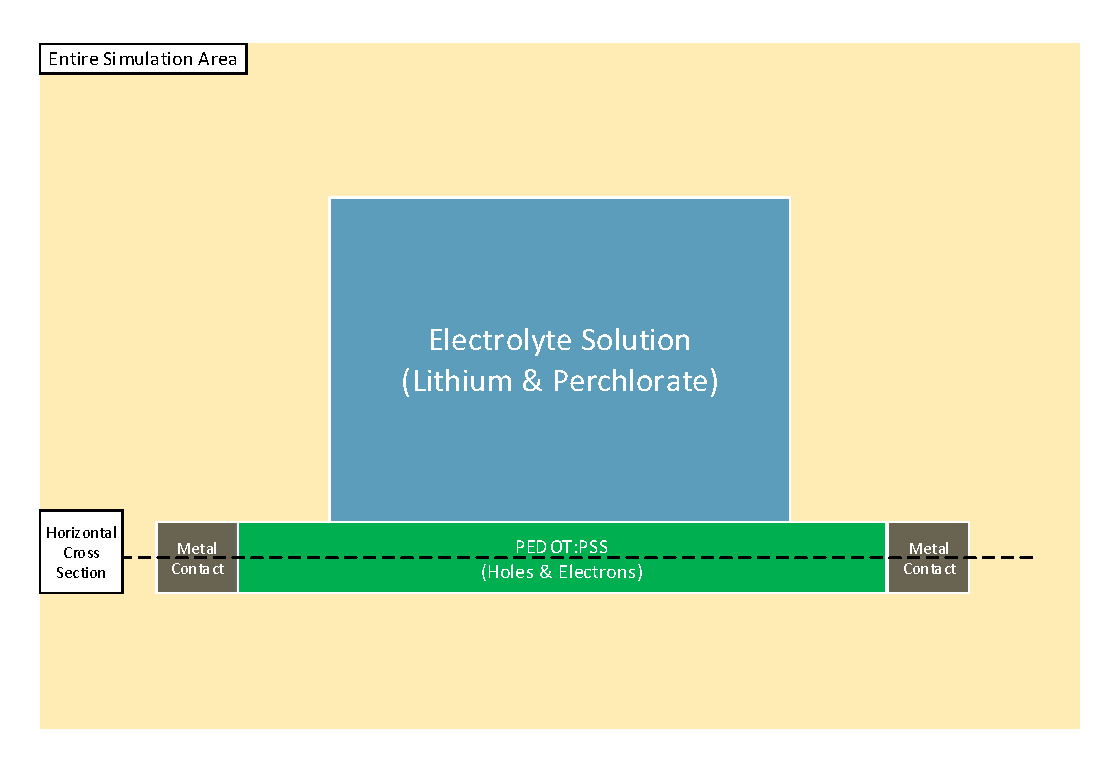
\includegraphics[scale=0.7]{Mem1}
\caption{The structure of the memristor used for simulation (not to scale)} 
\label{MemStc}
\end{figure}


The initial conditions for all the charge carriers are the same. All charges are balanced and uniformly distributed but the carrier density in the electrolyte solution is higher than the carrier density in PEDOT:PSS. Perchlorate ions are not allowed to move outside the electrolyte solution so a no flow boundary condition is used around the electrolyte. Lithium ions are free to move between PEDOT:PSS and the electrolyte solution but their maximum concentration is limited inside the PEDOT:PSS. The mobility of lithium ions has further restrictions inside PEDOT:PSS. Lithium has higher mobility in PEDOT:PSS right under the electrolyte solution, wet PEDOT:PSS, than the region without any contact with electrolyte, dry PEDOT:PSS. In fact due to this difference very little amount of lithium reaches the metal contacts. This decrease in mobility was modeled by making the mobility of lithium a function of position in PEDOT:PSS. The mobility of lithium ions were assumed to be 100 times slower than the mobility of holes in the wet PEDOT:PSS and it is zero in the dry PEDOT:PSS( $\mu_{hole} \approx$ $10^{-3}$ $m^2/Vs$). 


PEDOT:PSS is a regular conductor with fixed negative charge and mobile holes. Holes can move in an out of the PEDOT:PSS through the metal contacts which hold the charge neutrality of the initial condition throughout the simulation. The interface between PEDOT and electrolyte only allows the exchange of lithium ions. During simulation,the movement of lithium ions changes the conductivity of the PEDOT:PSS by increasing or decreasing the amount of available holes through coulomb forces. In the actual device lithium ions also change the conductivity via various physical effects like changing the mobility of holes through modifying their hopping distance. Even though the mobility of the holes can simply be made a function of the lithium density, the shape of the function is not known. The physical details of these additional effects are beyond the scope of this thesis. 




\clearpage
\section{Simulation Requirements}

It is important to analyze computational requirements of a simulation in order to asses the feasibility of the computation scheme. In this case, it is possible to determine the spacial and the temporal requirements using the equations \ref{debye} and \ref{CFL_Drift} which describe physical and numerical limitations of the simulation. Following graph \ref{SpaceTime} shows the requirements for a memristor of the scale discussed above and a typical semiconductor device size around 1 $\mu$m. The mesh density has to be high enough in order to capture the exponential charge accumulation for charge shielding so the minimum step size was set to be 5 times smaller than the Debye length. Plots \ref{SpaceTime}.a and \ref{SpaceTime}.c show the amount of points required to simulate a semiconductor and a memristor based on minimum step size. It is important to note that these values are for 1-D simulation and they can be converted to 2-D and 3-D by squaring or cubing y axis values respectively. Plots \ref{SpaceTime}.b and \ref{SpaceTime}.d are created using CFL conditions for drift and diffusion and dielectric relaxation time. A typical simulation time is estimated using mobility and electric field. Based on the estimated simulation time the number of time steps are calculated using the minimum time step obtained from CFL conditions and dielectric relaxation time.

It can be seen from graphs \ref{SpaceTime}.a and \ref{SpaceTime}.c that memristor simulations require much higher mesh densities compared to a typical semiconductor simulation such as 1 $\mu$m long PN diode. This is due to the larger size and higher charge density of the memristor. Graph \ref{SpaceTime}.a \ref{SpaceTime}.b show that a memristor with $10^{26}$ $m^{-3}$ charge density of the electrolyte would require close to $10^9$ points and $10^{14}$ time steps to simulate in 1-D. These requirements make the simulation of the memristor extremely challenging. In order investigate and find possible solutions for this issue, first a memristor with low charge density ($\approx 10^{15}$) was simulated in order to ensure that the simulation functions as designed. Then memristors with different charge densities were simulated and compared with each other to asses whether the behavior at low charge densities will be comparable to behavior at high charge densities.

\begin{landscape}
\begin{figure}[htp]
\centering
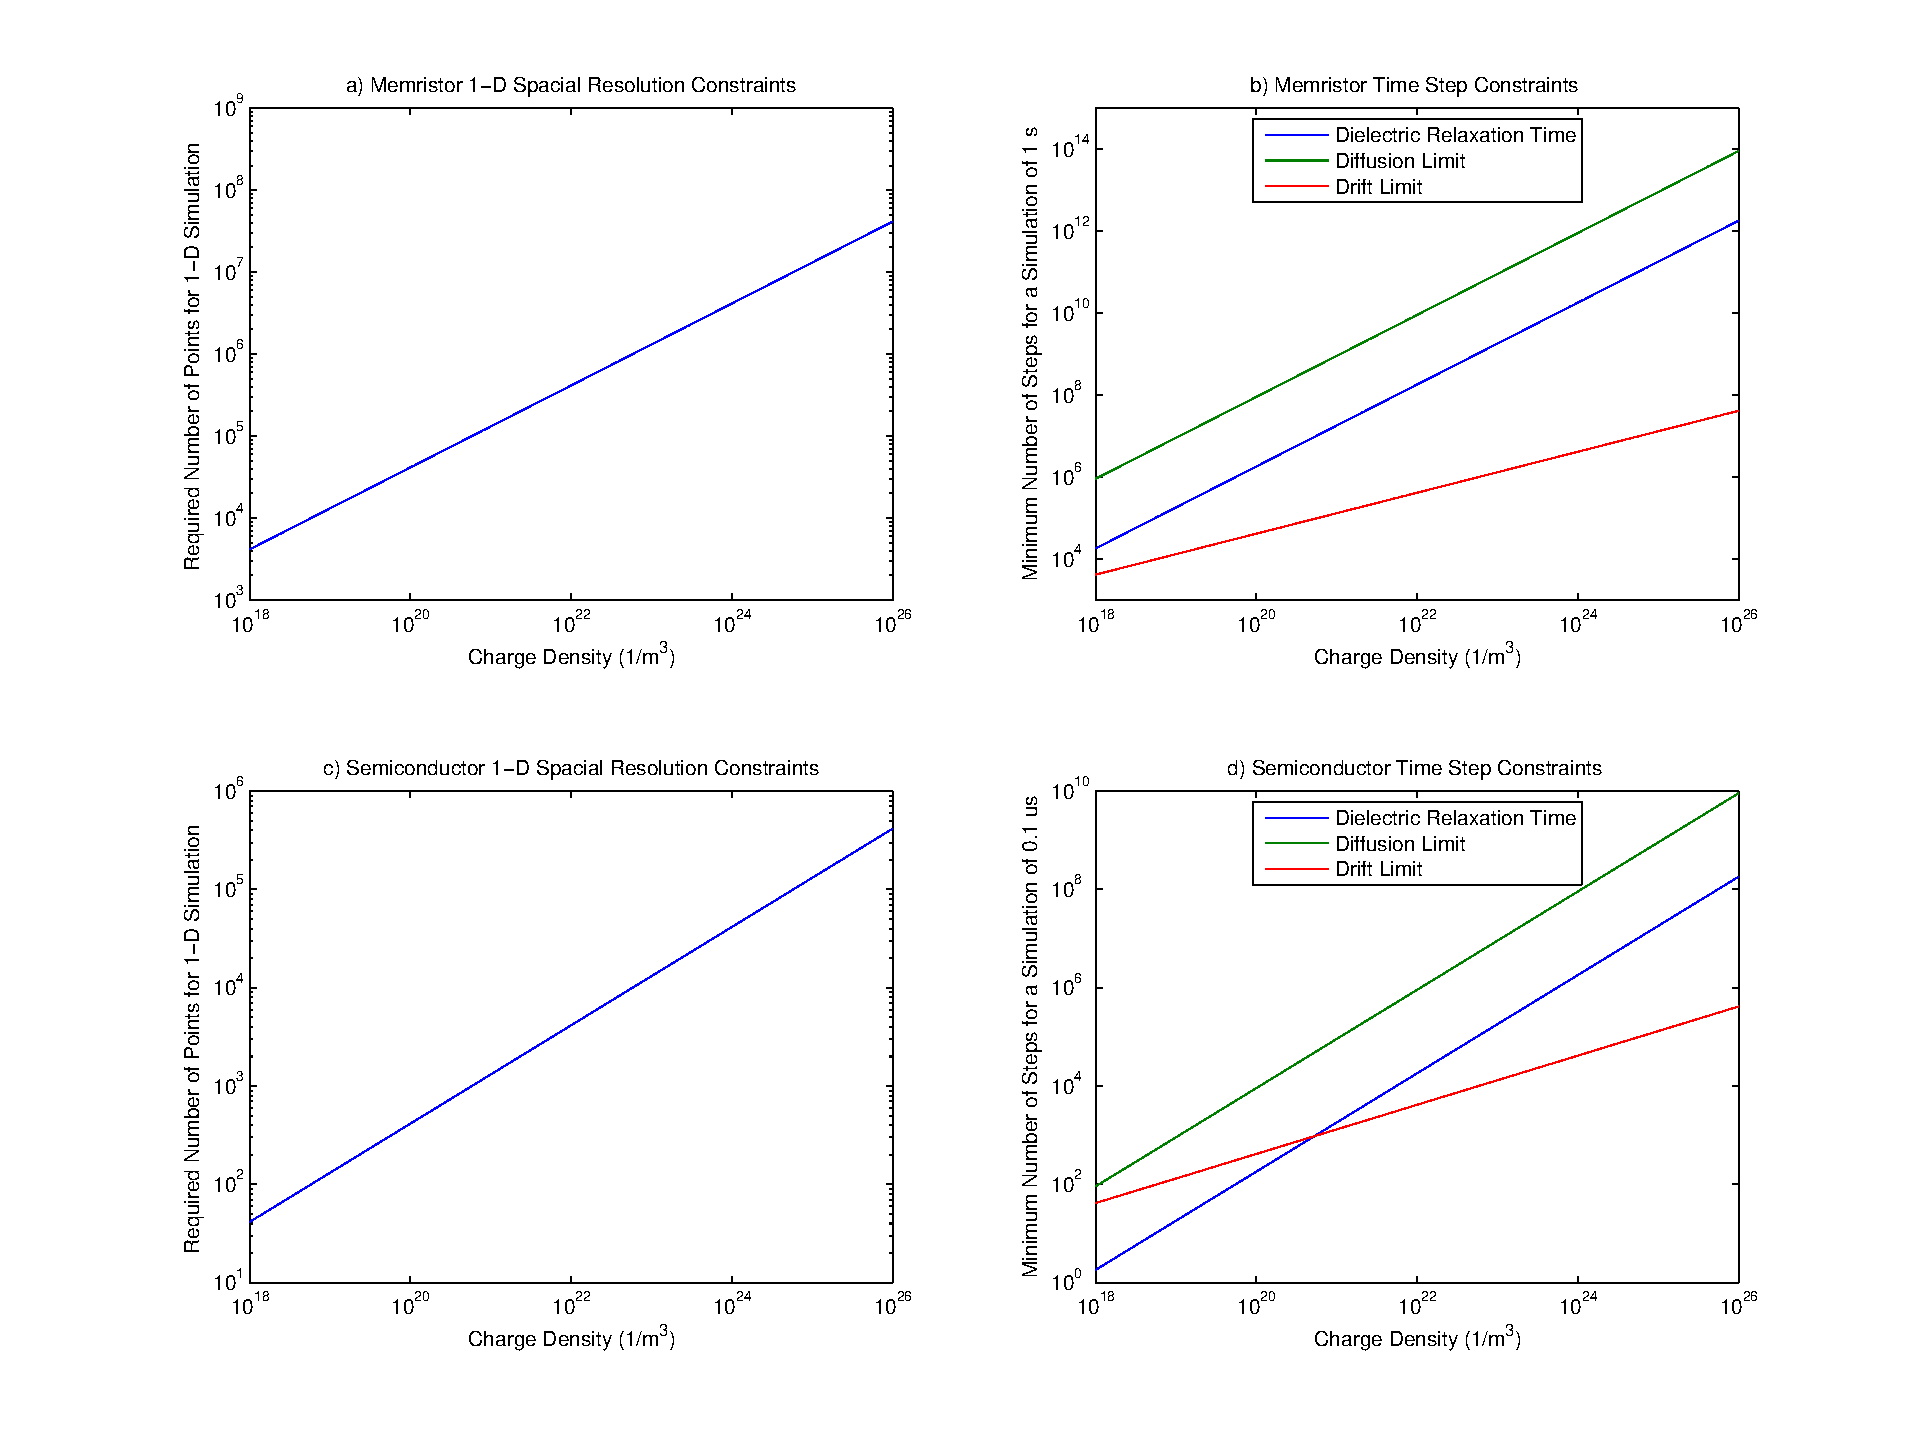
\includegraphics[scale=0.60]{SpaceTime}
\caption{Spatial and temporal requirements for simulation} 
\label{SpaceTime}
\end{figure}
\end{landscape}


\clearpage
\section{1-D Memristor Approximation}

The horizontal cross section from figure \ref{MemStc} has the most crucial elements of the memristor but its simulation in 1-D is not straight forward. This cross section through the PEDOT does not include the vertical movement of lithium. Without this effect, PEDOT is just a regular conductor with a uniform current density. In order to overcome this problem a generation/recombination term for lithium ions, calculated at every time step, was added to capture the vertical movement in addition to regular drift diffusion equations which represents the horizontal movement. This generation/recombination term can be symbolized as a current source with a resistor connected to all the nodes (figure \ref{MemStc15}). Perchlorate ions were not included in the simulation since they do not move into the PEDOT.

\begin{figure}[!htp]
\centering
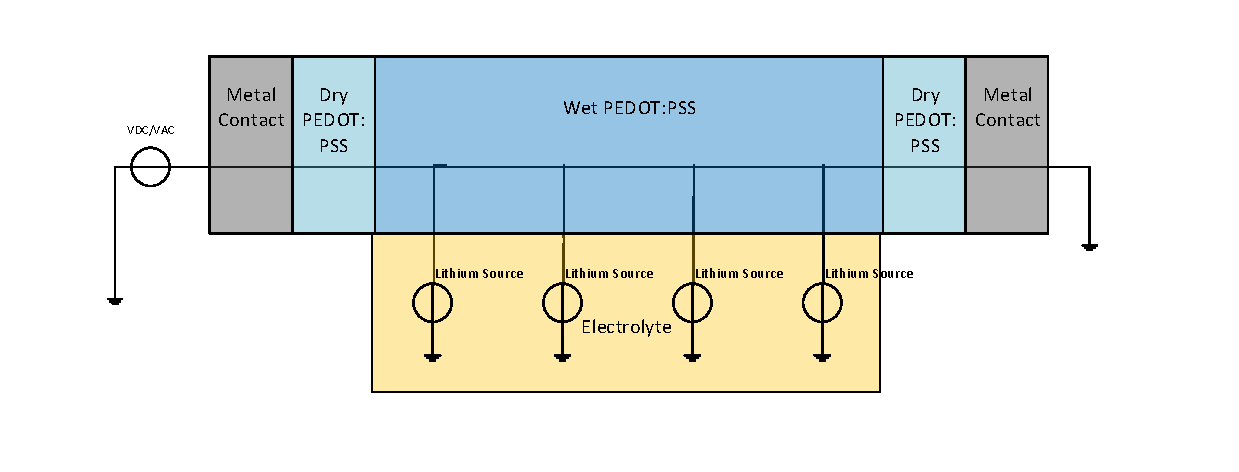
\includegraphics[scale=0.74]{1DMem}
\caption{1.5-D Memristor Structure} 
\label{MemStc15}
\end{figure}

The lithium source has two different terms, one for drift and another one for diffusion. It was assumed that the concentration of lithium is always constant in the electrolyte. This way the vertical diffusion current density can be calculated using the difference between the lithium density in PEDOT and electrolyte. For the diffusion term an electric field is estimated between the PEDOT and the electrolyte. First the potential of the electrolyte is assumed to be half of the net applied potential. Then an electric field is calculated using the electrolyte and the instantaneous potential of the PEDOT at different positions.

Since the main characteristic of memristor is the change in resistivity over time it is important to develop a standard approach for measuring the resistivity. Initially, simulations in this chapter and the following one, were run until steady state without the movement of lithium/perchlorate ions. Ions in the electrolyte start to move after the steady state has been reached. The movement of ions create another transient which involves changes in resistivity. The current density (at steady state) obtained from the initial simulation was used as a normalizing factor in order to determine the changes in resistivity after the ion movement has started.

\clearpage
\section{1-D Memristor Simulations}

Following simulations were made based on the memristor approximations discussed above. First two simulations are repeated in the next chapter using a 2-D drift diffusion and Poisson solver which captures a broader range of physical effects. Both approaches can be compared in order to understand their advantages and disadvantages under different circumstances.

\subsection{1-D Memristor Simulation Using a Potential Pulse Train}
  
For the following simulation a potential pulse train, slow enough to let the memristor reach steady state, was applied at the left contact. Following plot \ref{MemResTrain} shows the resistivity measured using both contacts separately. As expected the resistance of the device more than doubled as the lithium ions move in. Additionally, it can be seen from the graph \ref{MemResTrain} that the resistivity measurements from left and right contacts are not always the same over the duration of the simulation. This is normal since it is due to PEDOT layer losing holes on one side and gaining holes on the other which produces a difference in measured resistivity between contacts. The scale of the difference depends on the rate of change in resistivity on one side. When holes are not fast enough to track the change in resistivity, the current on each side take different values.  

\begin{figure}[!htp]
\centering
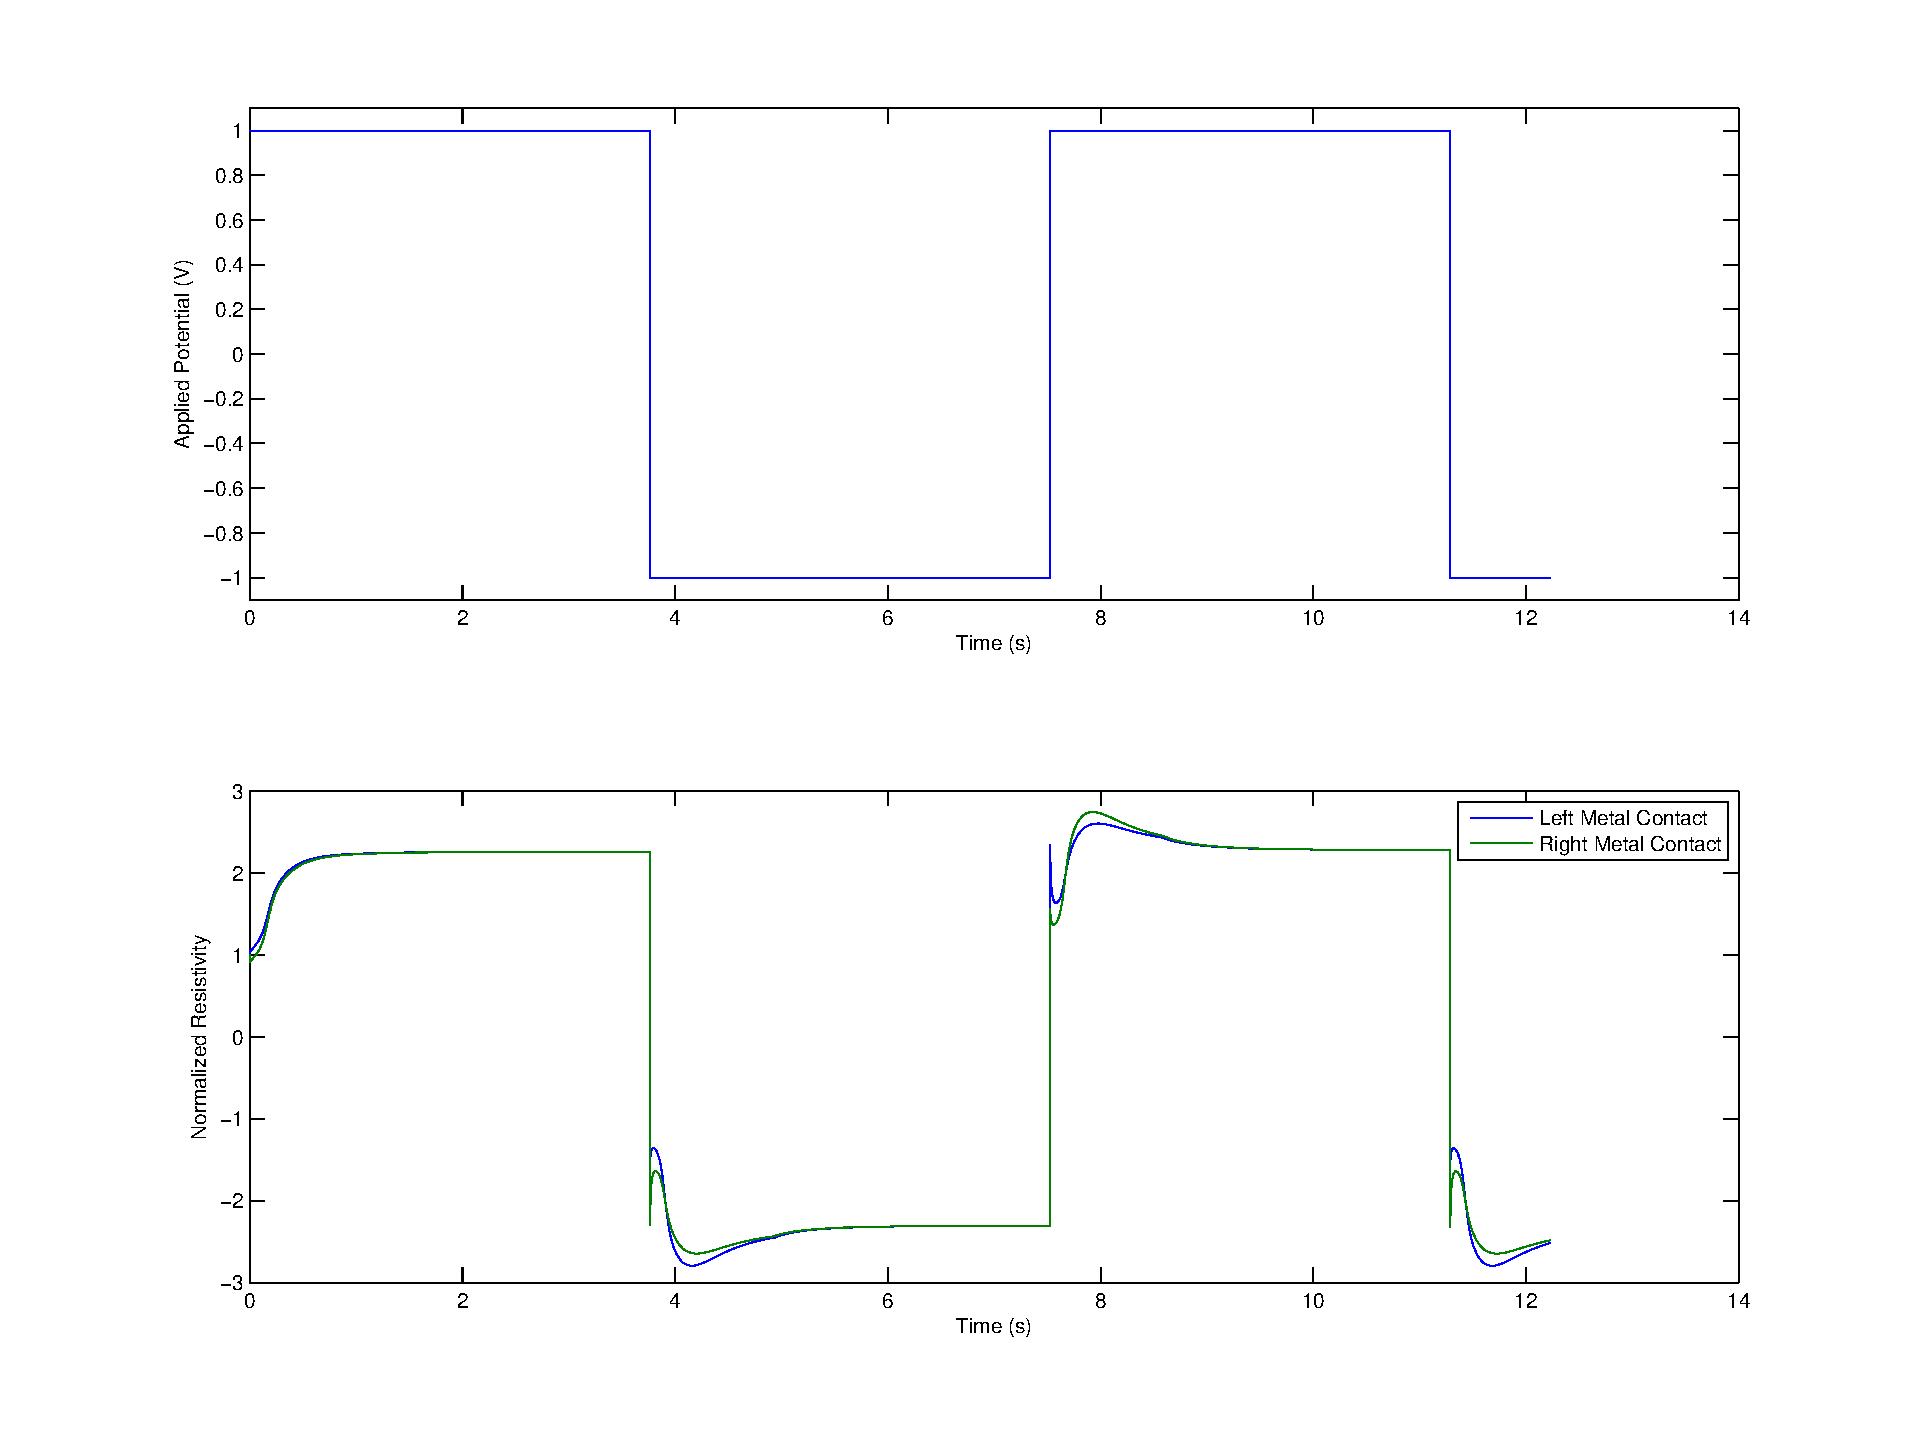
\includegraphics[scale=0.40]{1DMemPulseTrain}
%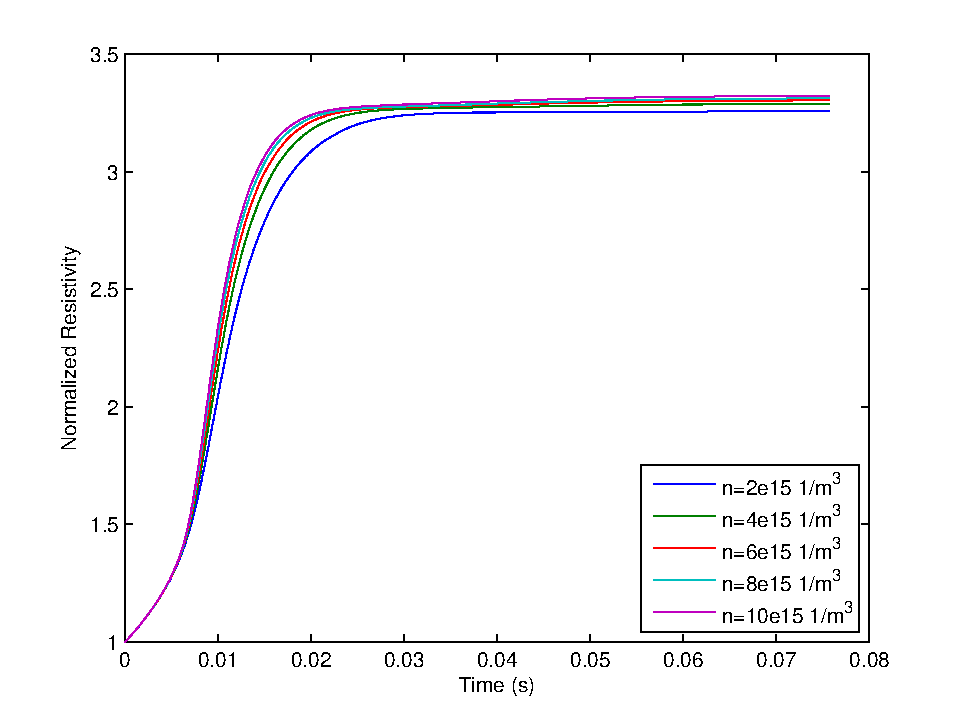
\includegraphics[scale=0.60]{Ex5DCResistivity}
\caption{Change in resistivity over time due to applied potential} 
\label{MemResTrain}
\end{figure}

The resistivity in figure \ref{MemResTrain} shows a sudden drop when the potential is switched from 1 to 0 and vice versa. This sudden drop occurs because of the accumulation of lithium ions and holes near the negative contact which opposes the electric field generated due to the applied potential (see figure \ref{MemEss}). When the potential changes suddenly, previously opposing electric field now helps the movement of holes and lithium towards the other end of the device. This additional electric field momentarily reduces the resistivity of the device.

\begin{figure}[!htp]
\centering
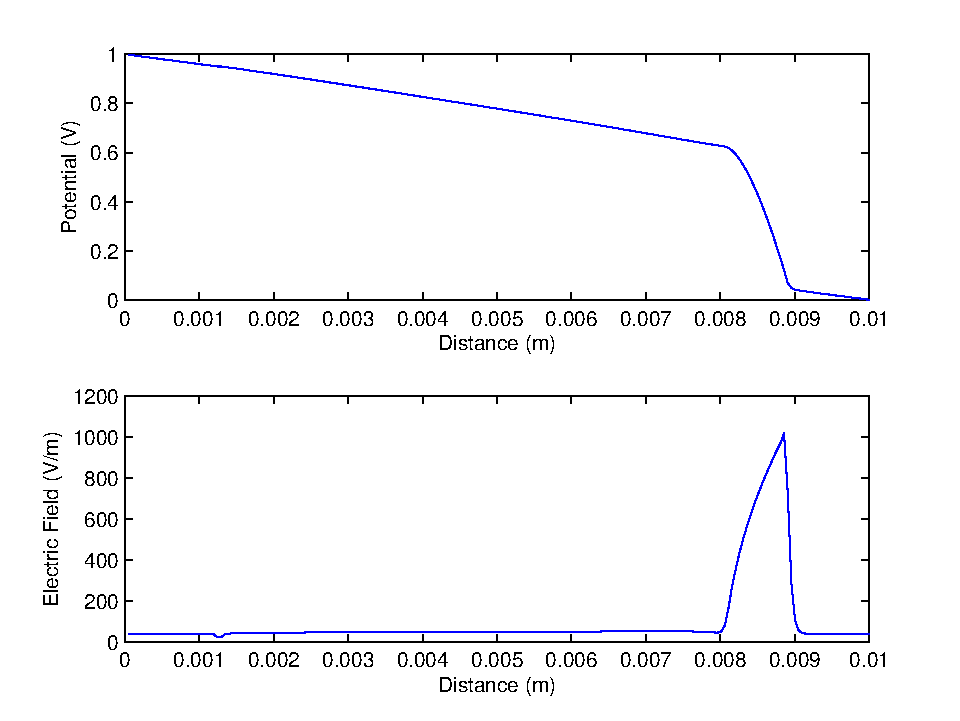
\includegraphics[scale=0.70]{1DMemPot_Efield_SS}
\caption{Potential and electric field at steady state} 
\label{MemEss}
\end{figure}

Figure \ref{MempLi} demonstrates the replacement of holes by lithium ions over time which directly effects resistivity seen in figure \ref{MemResistivityTrain}.  As lithium ions get pulled in from the electrolyte toward the contact they accumulate inside PEDOT and push holes out via coulomb forces. Decreased hole concentration in the PEDOT increases the resistivity of the material. This change in resistivity over time is illustrated in figure \ref{MemResTrain}.

\begin{figure}[!htp]
\centering
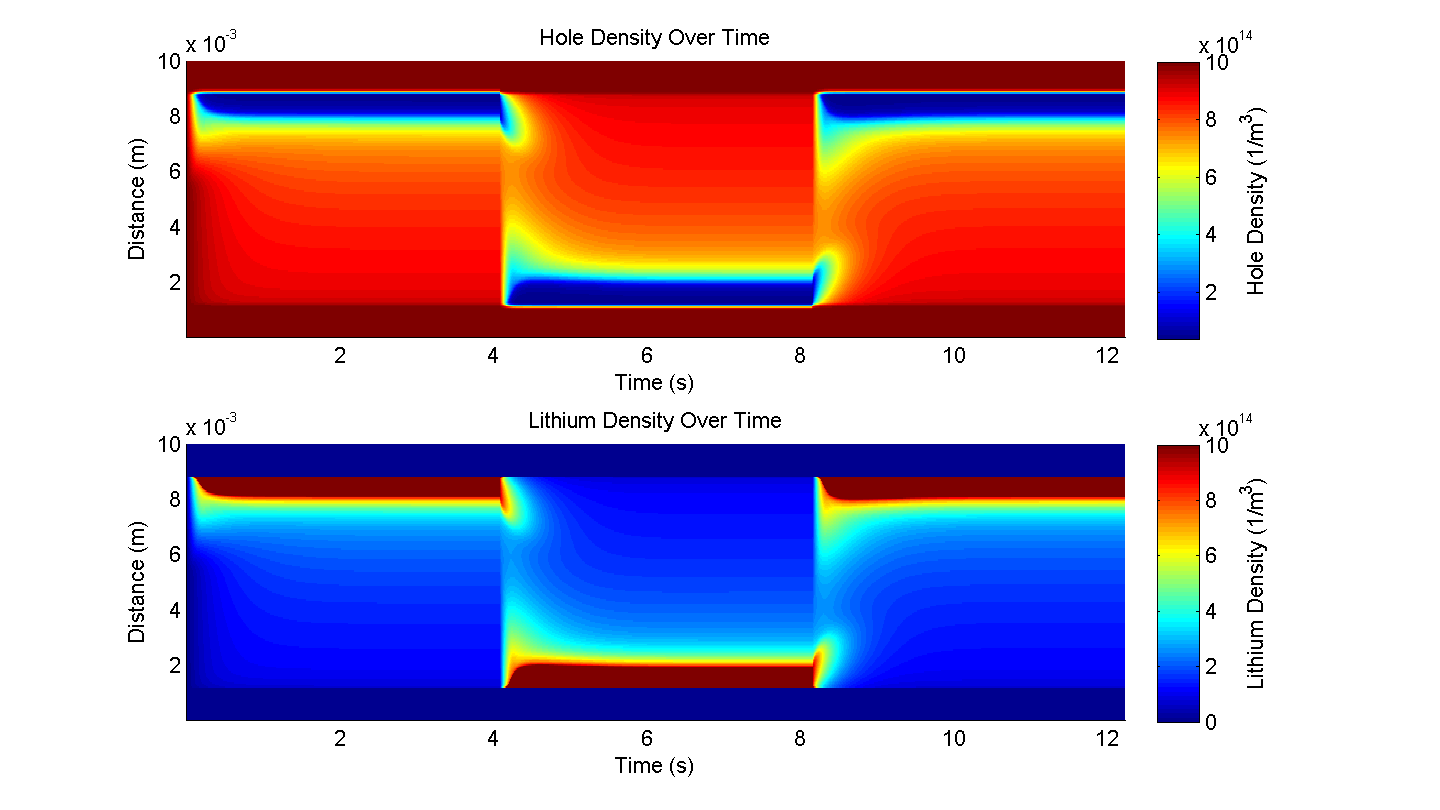
\includegraphics[scale=0.65]{1DMemDensityOverTime}
%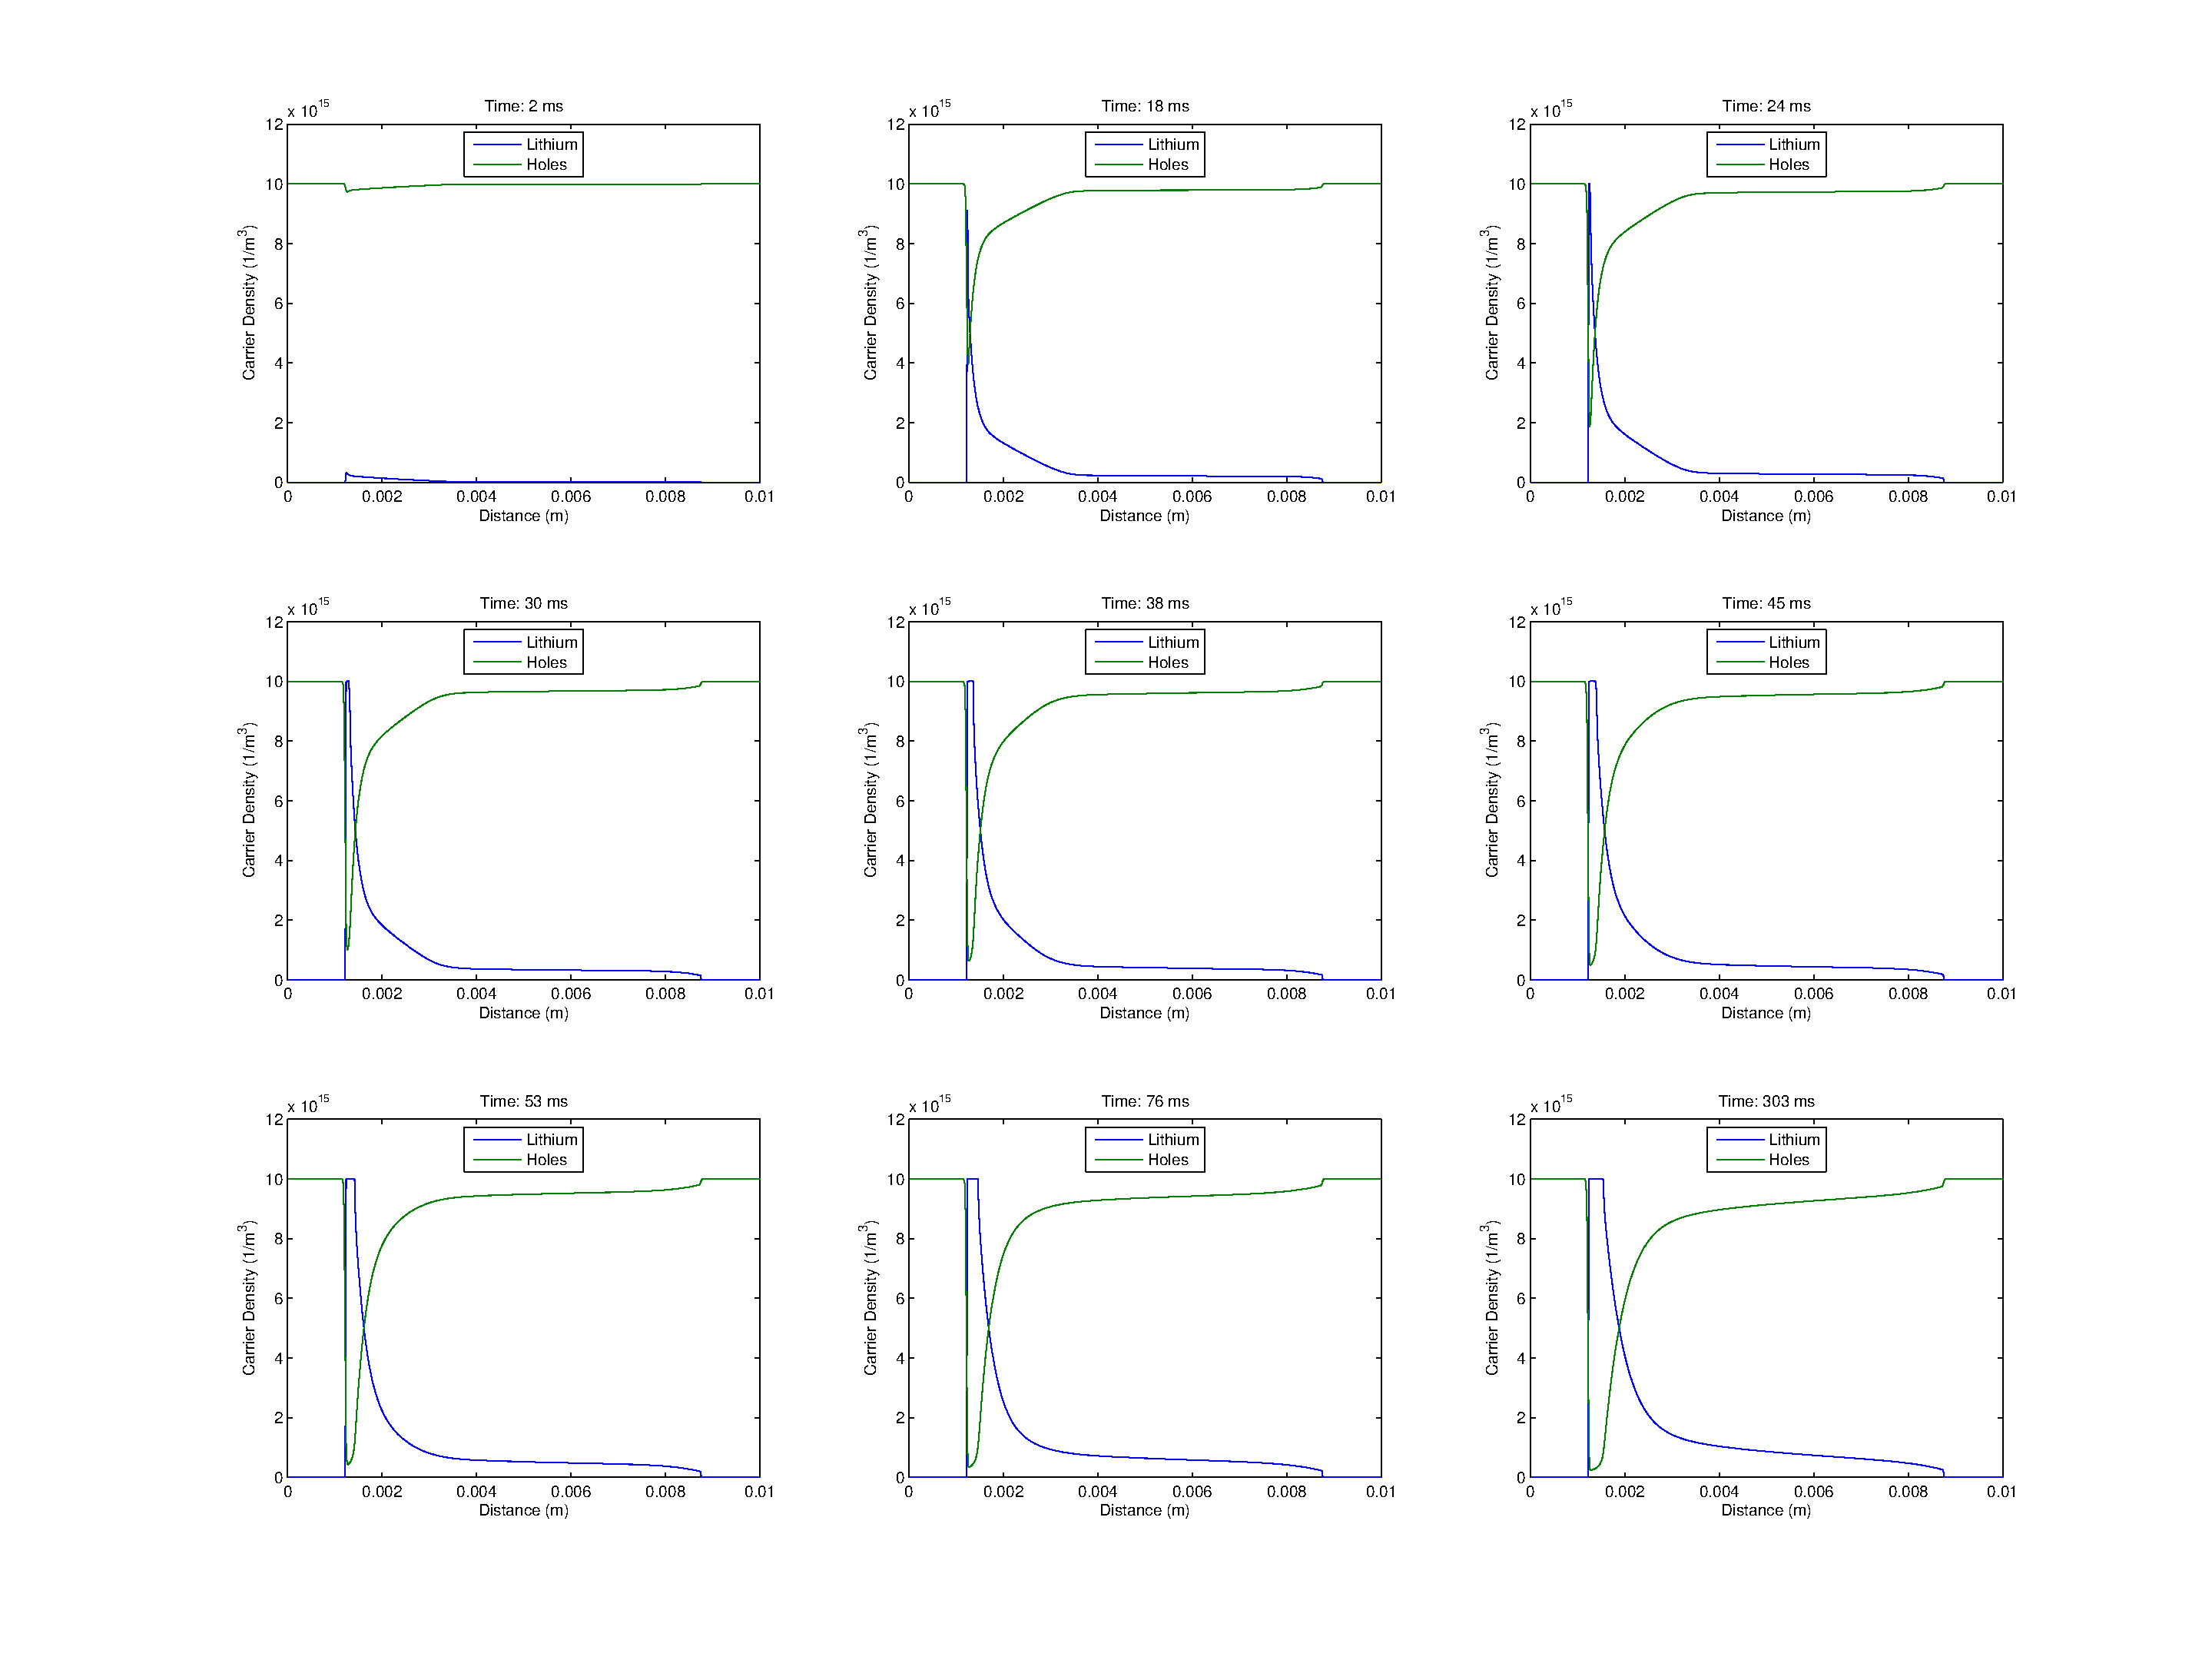
\includegraphics[scale=0.40]{Ex5pNp_Time1}
\caption{Lithium and hole density distribution over time} 
\label{MempLi}
\end{figure}

It is important to note that lithium ions are free to move in x and y direction. In figure \ref{MempLi} it can be seen that after the potential is switched as the lithium density moves from  side to the other. Most of the lithium movement happens through the exchange of ions between PEDOT and the electrolyte since the distance between them is far less than the length of the PEDOT. So lithium ions, traveling from the positive to the negative contact, are pulled into the electrolyte before they reach the other side. Near the negative contact lithium ions are quickly pulled into the PEDOT and accumulate at the wet/dry interface. Figure \ref{MemResistivityTrain} shows the changes in resistivity throughout PEDOT due to the accumulation of lithium. The resistivity is increased in regions where there is high lithium accumulation. 

By examining the resistivity plot of PEDOT it is possible to conclude that it is composed of 3 distinct regions. 2 dry regions, where there is no contact with the electrolyte, have constant uniform resistance. Between these two resistances there is a variable non uniformly distributed resistance controlled by hole/lithium concentration and hole mobility. So this model captures the main characteristic of the memristor which is a variable resistance where the resistance at any time depends on the past of the device. Following equation gives the total resistance/memristance for the memristor model developed for this thesis:

\begin{equation}
\centering
M(q(t))_{tot}=2R_{dry}+R(Li,p,\mu_{hole})
\end{equation}

The minimum resistance of this device is just the total resistance of the PEDOT without the lithium ions. The maximum resistance depends on different factors such as applied potential and the distribution and concentration of lithium ions inside PEDOT.

\begin{figure}[!htp]
\centering
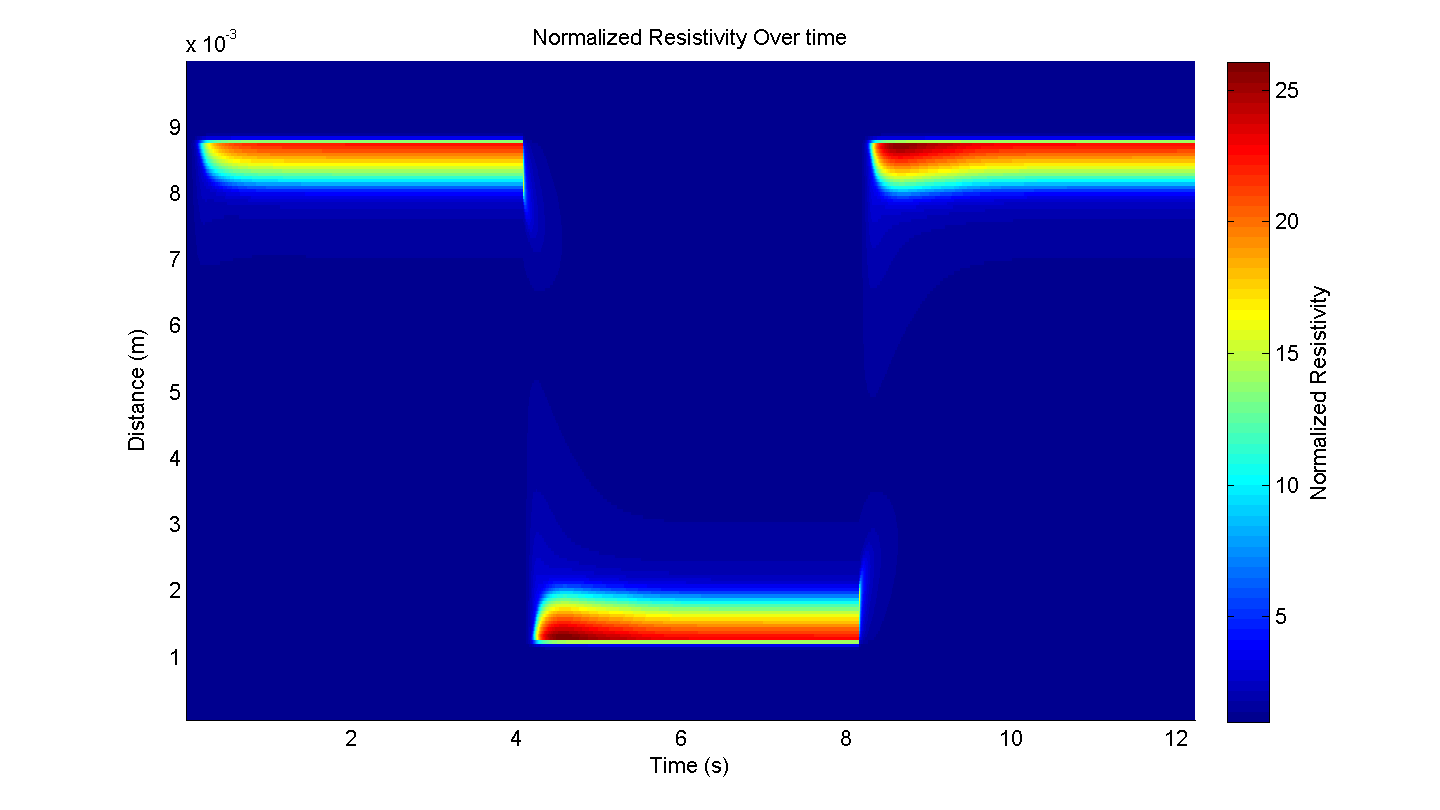
\includegraphics[scale=0.65]{1DMemResistivityOverTime}
\caption{Normalized resistivity over time} 
\label{MemResistivityTrain}
\end{figure}

\clearpage
\subsection{1-D Memristor Simulation Using a Sinusoid}

Memristor with a pulse train simulation shows the change in resistivity over time due to an applied potential but it does not clearly demnostrate memory effects. The memory effect of the memristor can be clearly demonstrated in an I-V curve using sinusoidal potential. Following four graphs (figure \ref{Bowtie}) were created using an AC potential with different frequencies at the contacts. All the plots show that current can have more than one value for the same potential at different times. This means that simulated memristor's past states affects its present output, therefore the device has memory. There is a pinch in the current for negative applied potential because it is measured from one contact which sees a higher resistance for a period of time during transient. 

\begin{figure}[!htp]
\centering
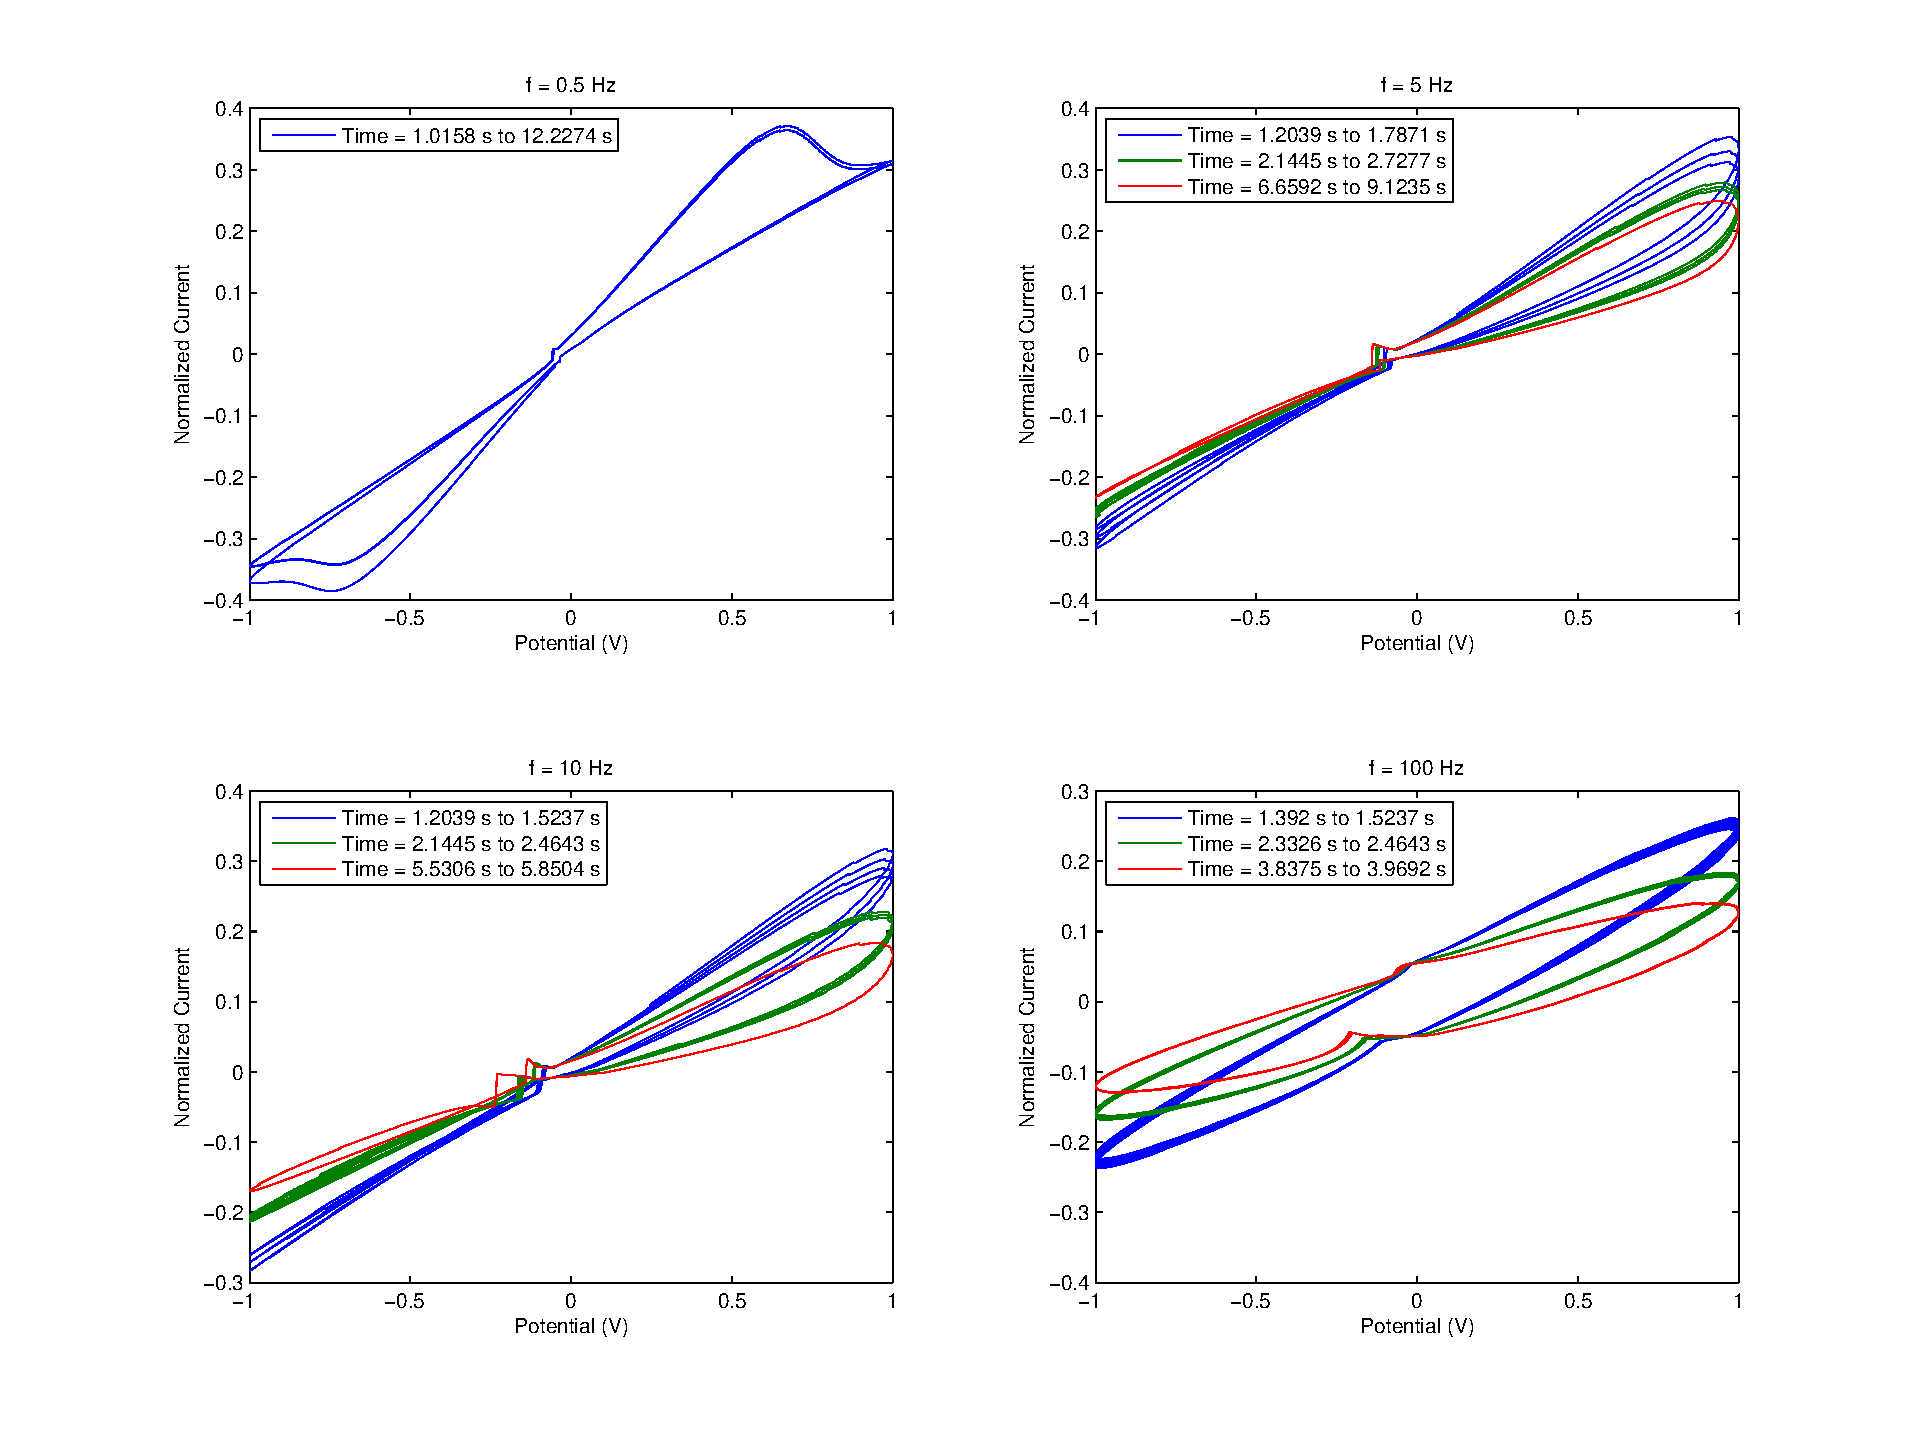
\includegraphics[scale=0.45]{BowtiefAll}
\caption{Normalized Current vs. applied potential at different frequencies} 
\label{Bowtie}
\end{figure}


The sudden changes in current around 0 V can be attributed to the density limiting mechanism for lithium. Instead of a slowdown in the movement of lithium ions near maximum concentration, the current flow into that region is completely blocked. Even though this makes the lithium density more responsive to changes, sudden movement block combined with large time steps can result in fast changes which can be directly seen as abrupt changes in the hole/lithium current density during transient simulations.  

As AC potential pushes lithium ions from one side to the other, an equilibrium is reached over time. The change in resistivity starts to repeat itself and after a while it becomes  periodic. Figure \ref{BowtieCurr} shows the changes in memristor current over time for the right metal contact. At first, as lithium moves into the PEDOT there is a drop in current on average. Once enough lithium settles into the PEDOT, high resistivity region simply shifts from left to right but it stays fairly constant on average. 

\begin{figure}[!htp]
\centering
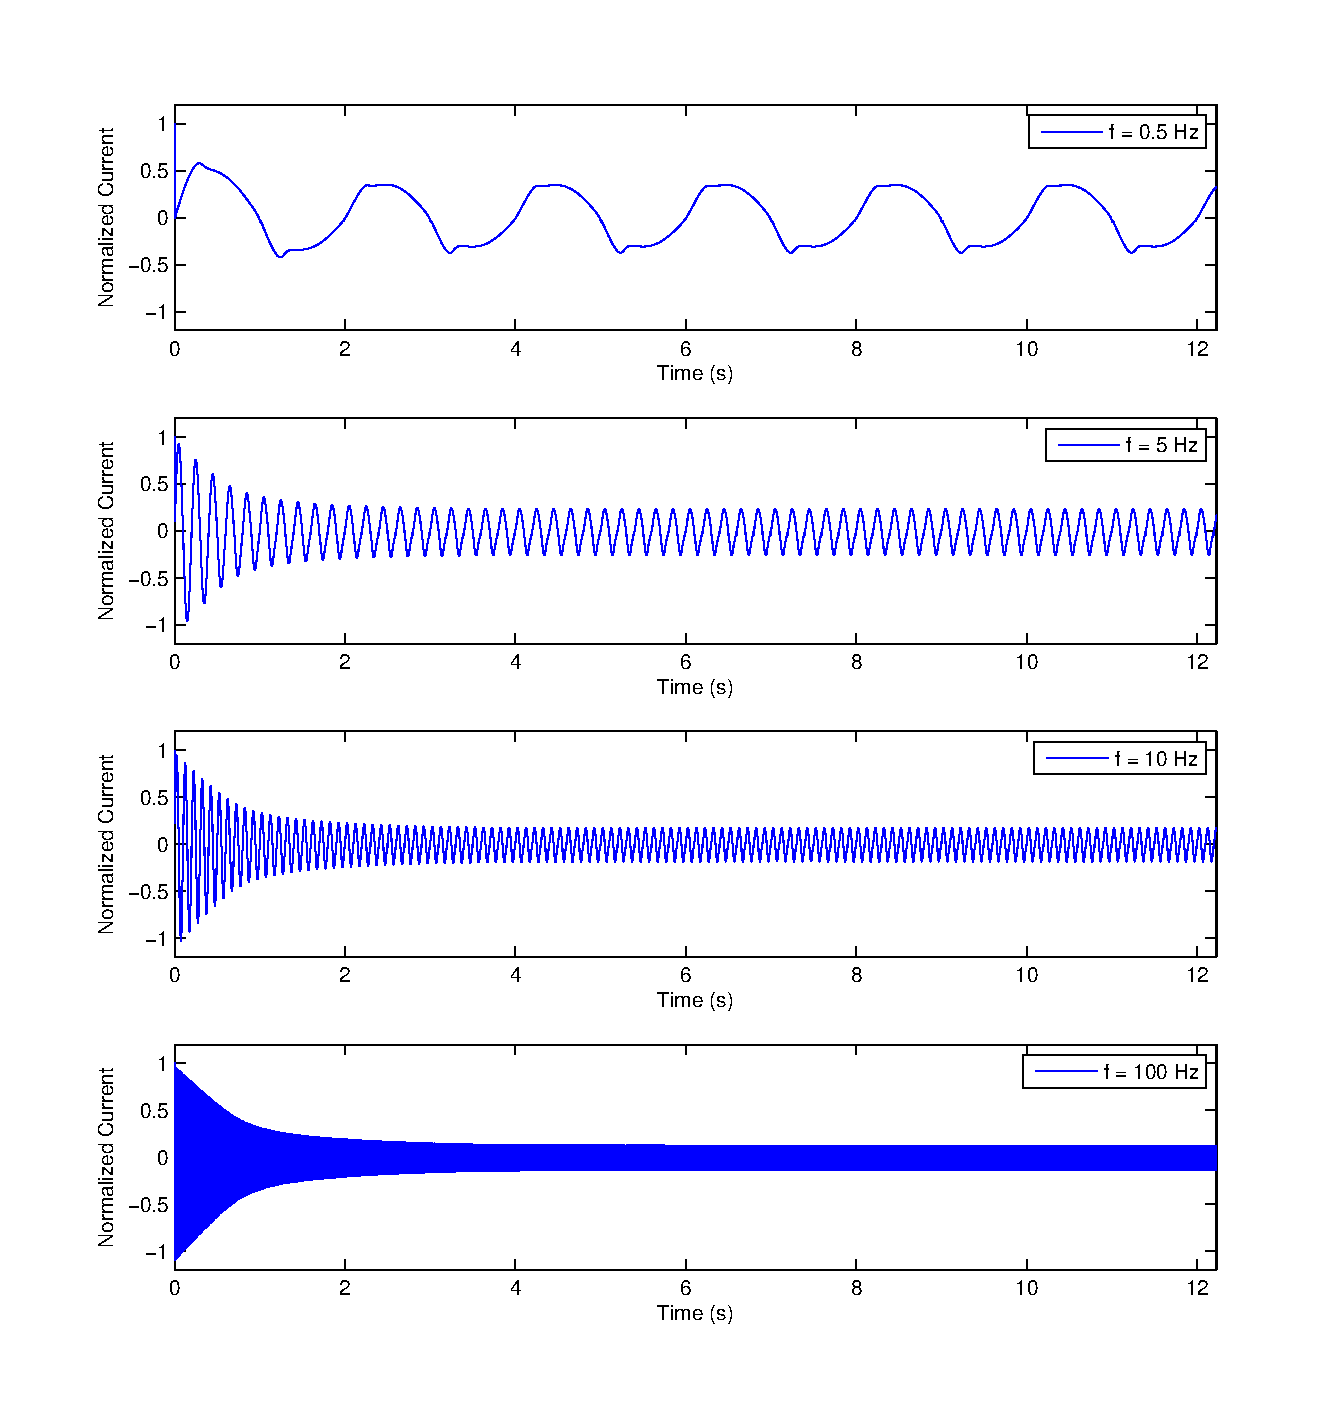
\includegraphics[scale=0.55]{BowtieCurr4f}
\caption{Normalized current over time} 
\label{BowtieCurr}
\end{figure}

Figures \ref{BowtieRes},\ref{Bowhole} and \ref{Bowli} show the changes in resistivity, hole and lithium density in PEDOT over time. A visual comparison of the plots show that changes in lithium density induces changes in hole density. As frequency increases diffusion becomes more dominant than drift. At 100 Hz drift due to applied potential is barely present. Since ions do not create a visible impact on the hole density, the resistivity of the device remains constant over time. This means that the memristor model behaves like a regular resistor at high frequencies.

\begin{figure}[!htp]
\centering
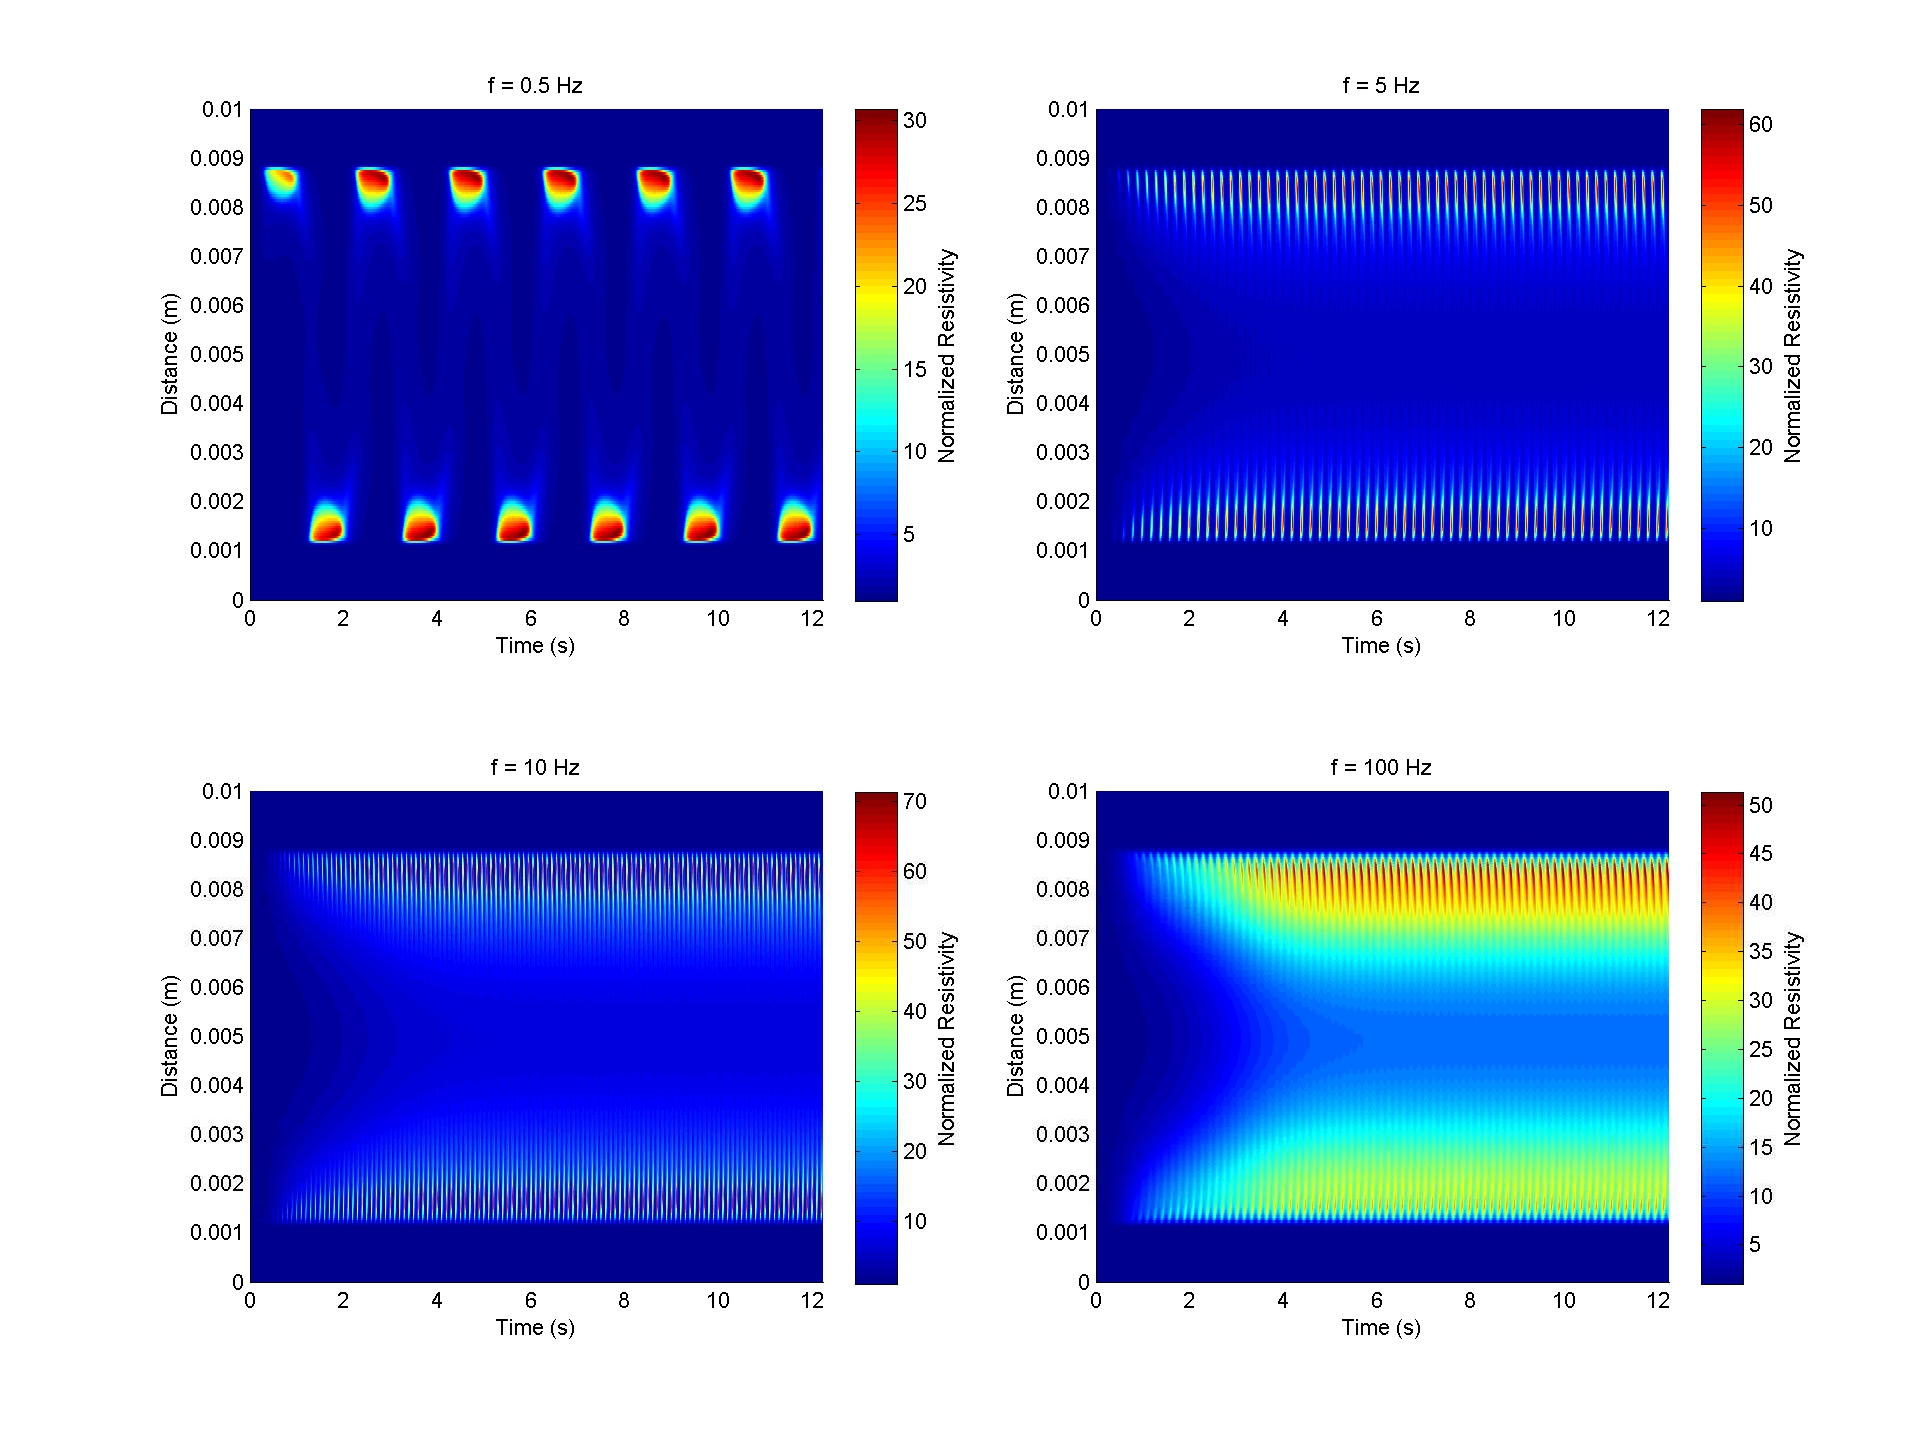
\includegraphics[scale=0.43]{1D_Memristor_Resistivity}
\caption{Normalized resistivity over time at different frequencies} 
\label{BowtieRes}
\end{figure}

\begin{figure}[!htp]
\centering
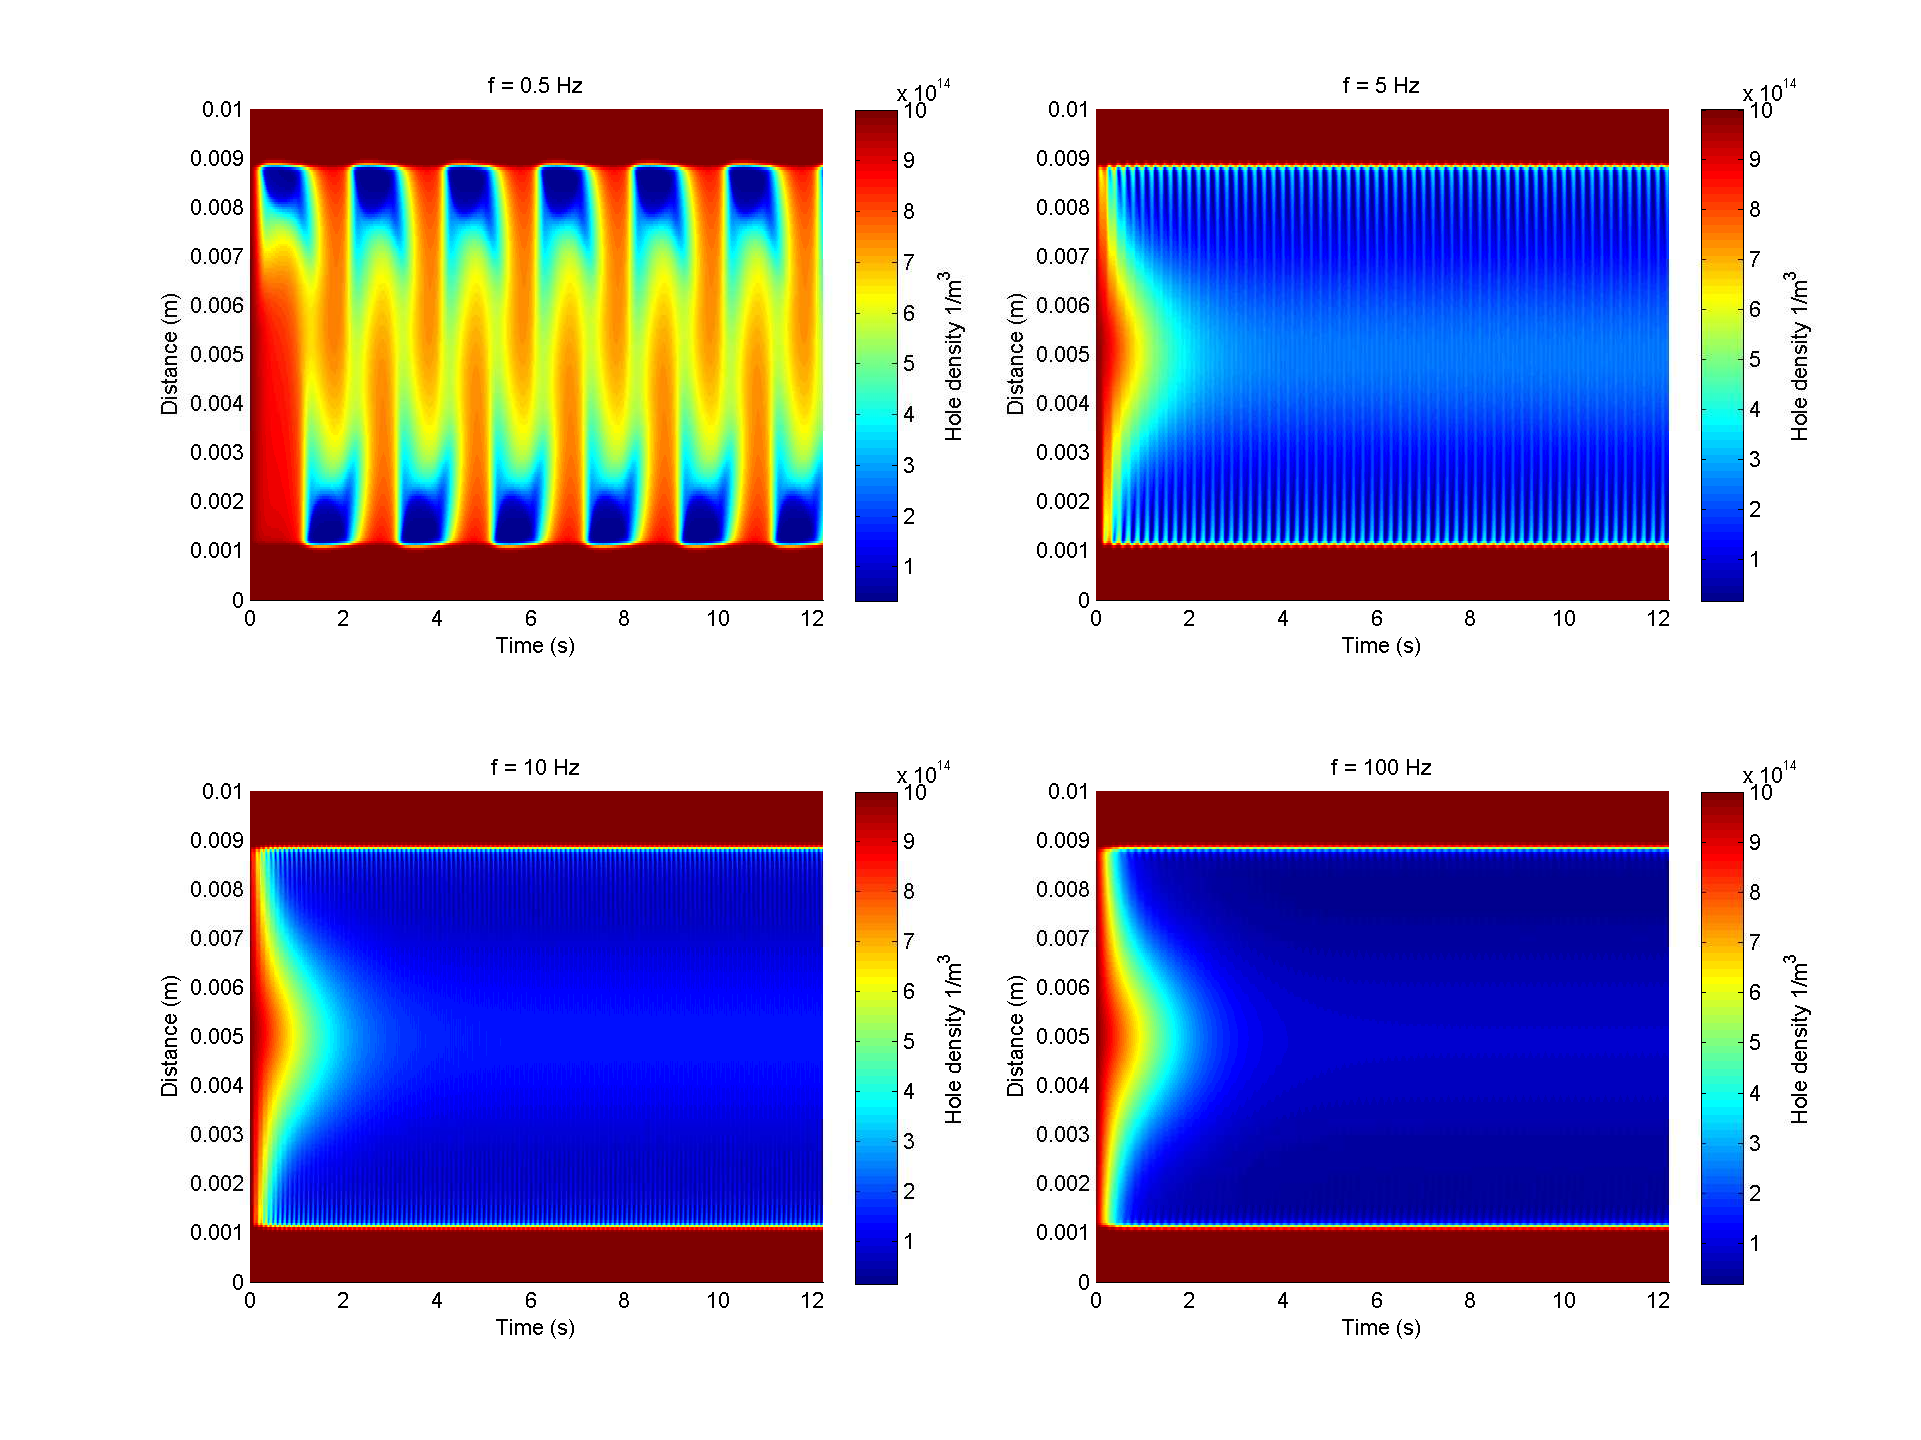
\includegraphics[scale=0.43]{1D_Memristor_Hole}
\caption{Hole density over time at different frequencies} 
\label{Bowhole}
\end{figure}



\begin{figure}[!htp]
\centering
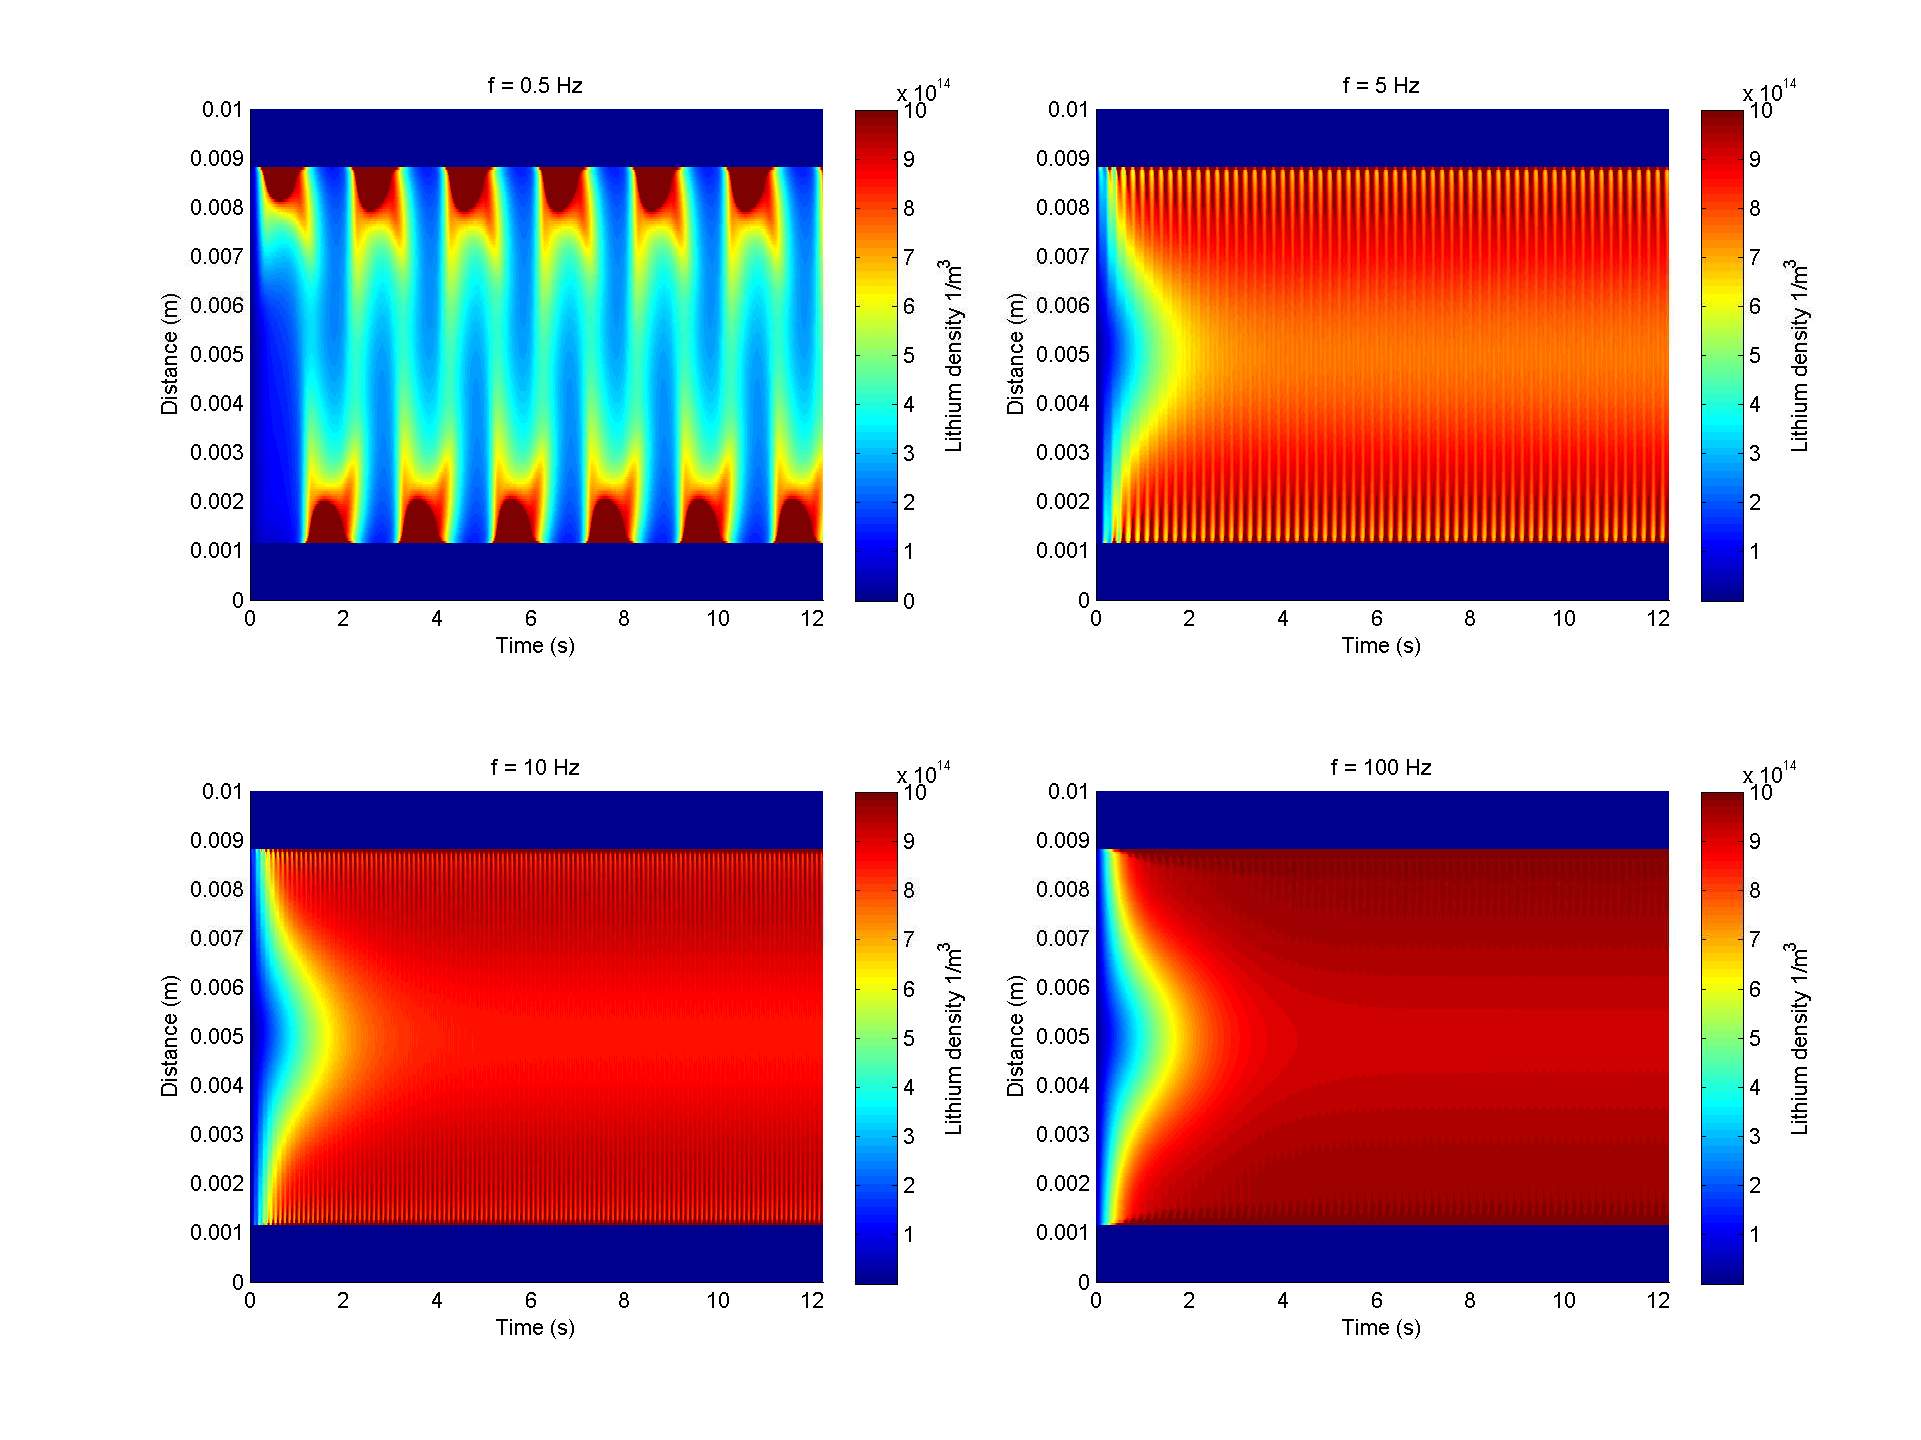
\includegraphics[scale=0.43]{1D_Memristor_Lithium}
\caption{Lithium density over time at different frequencies} 
\label{Bowli}
\end{figure}




\clearpage
\subsection{1-D Memristor Simulation With Increasing Charge Density}

After establishing that the simulation behaves as expected it is important to investigate how charge density effects this model since the size of the device limits the maximum charge density that can be simulated. The actual device has a hole density in the range of $ \approx 10^{22}$ $m^{-3}$ but the simulation is restricted to $\approx 10^{15}$ $m^{-3}$. In theory, if the densities used for simulation does have a limited affect on the behavior of the memristor then simulations in low densitiy can be use as a proxy for the actual device which operates in much higher carrier densities.

 Following 3 graphs (\ref{HoleDiff}, \ref{LithiumDiff} and \ref{DensityDiff} ) show hole and lithium densities at steady state as well as the current density over time at the right metal contact for various charge densities. The simulations were done on high mesh densities to allow stable simulation at high charge concentrations. 20 different simulations were made using densities ranging from $5$ x $10^{15}$  $m^{-3}$ to 1 x $10^{17}$  $m^{-3}$ but only 5 of them were plotted for illustration purposes. All the values were normalized to the initial plot using respective hole/lithium density ratios. Following equations were used for the normalization procedure.


\begin{equation}
\centering
n_{norm}= \frac{n_i}{r} 
\end{equation}
\begin{equation}
\centering
J_{norm}= \frac{J_i}{r} 
\end{equation}

\begin{equation}
\centering
r = \frac{n_{initial}}{n_{0}}
\label{NormConst}
\end{equation}

$n_{i}$ is the charge carrier density which could be either holes or lithium ions depending on the plot. J is the current density calculated from the right metal contact. r is the normalization constant which is calculated using initial carrier density ($n_{initial}$) of a simulation to be normalized and $n_{0}$ which is the carrier density of the initial plot ($5x10^{15}$ $m^{-3}$). After the normalization of various variables, all the plots were placed in the same graph to visually illustrate how increasing charge density affects the simulation. 

Plots for lithium ions (figure \ref{LithiumDiff}) and holes (figure \ref{HoleDiff}) are nearly identical to each other in terms of the plot shapes. They both get sharper around the area where there is a substantial accumulation of lithium. This is not unexpected since the debye length gets smaller with increasing carrier density concentration. So with increased density it is expected that the density accumulation at the wet/dry PEDOT interface will be more narrow. This affect is not as strong for lithium ions since there is a maximum concentration limit on them. Lithium and hole plots only show the difference carrier density makes at steady state. The affect of debye length on device operation can be further explored by looking at the current density over time.   

\begin{figure}[!htp]
\centering
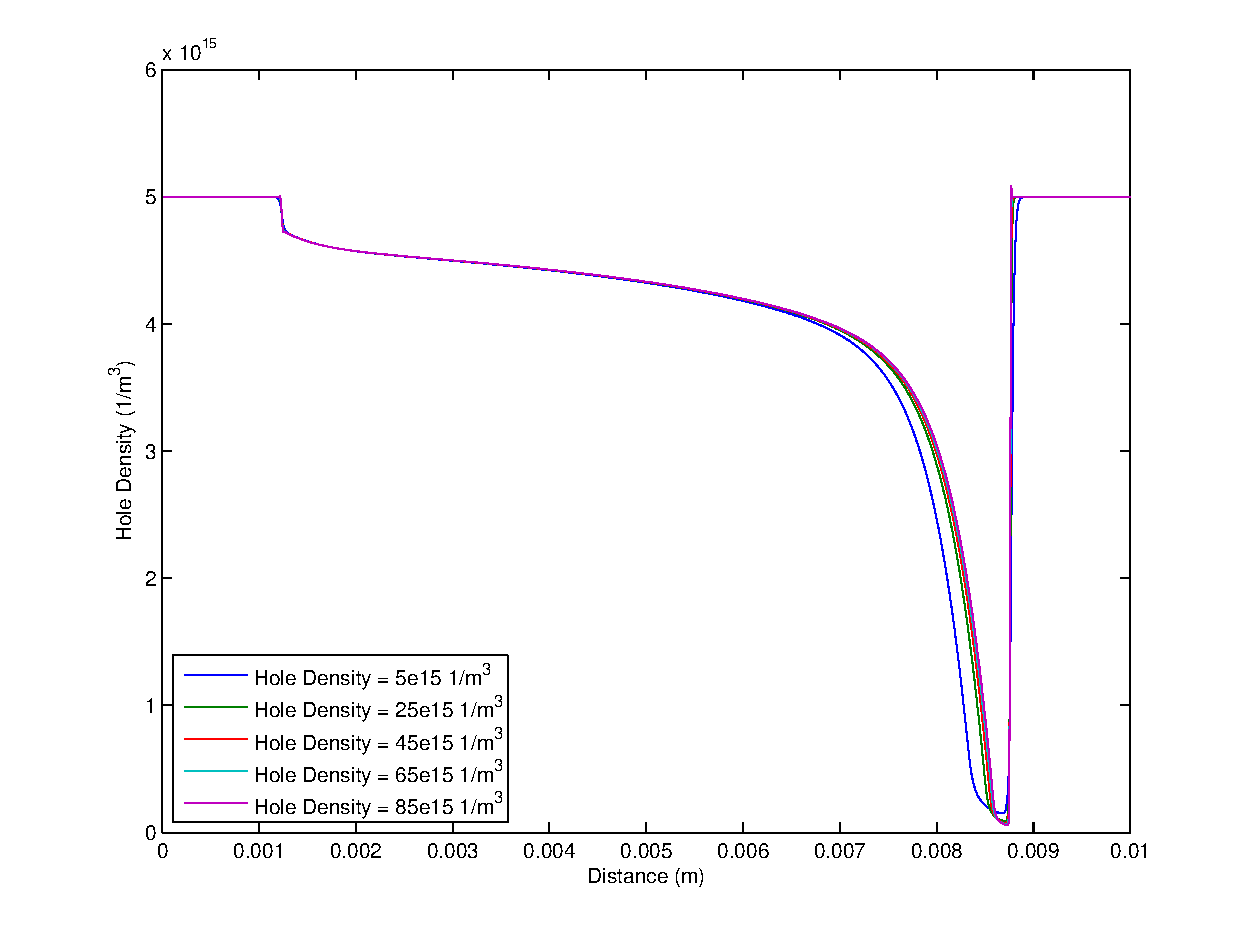
\includegraphics[scale=0.50]{HoleDiff}
\caption{Normalized hole densities at steady state} 
\label{HoleDiff}
\end{figure}

\begin{figure}[!htp]
\centering
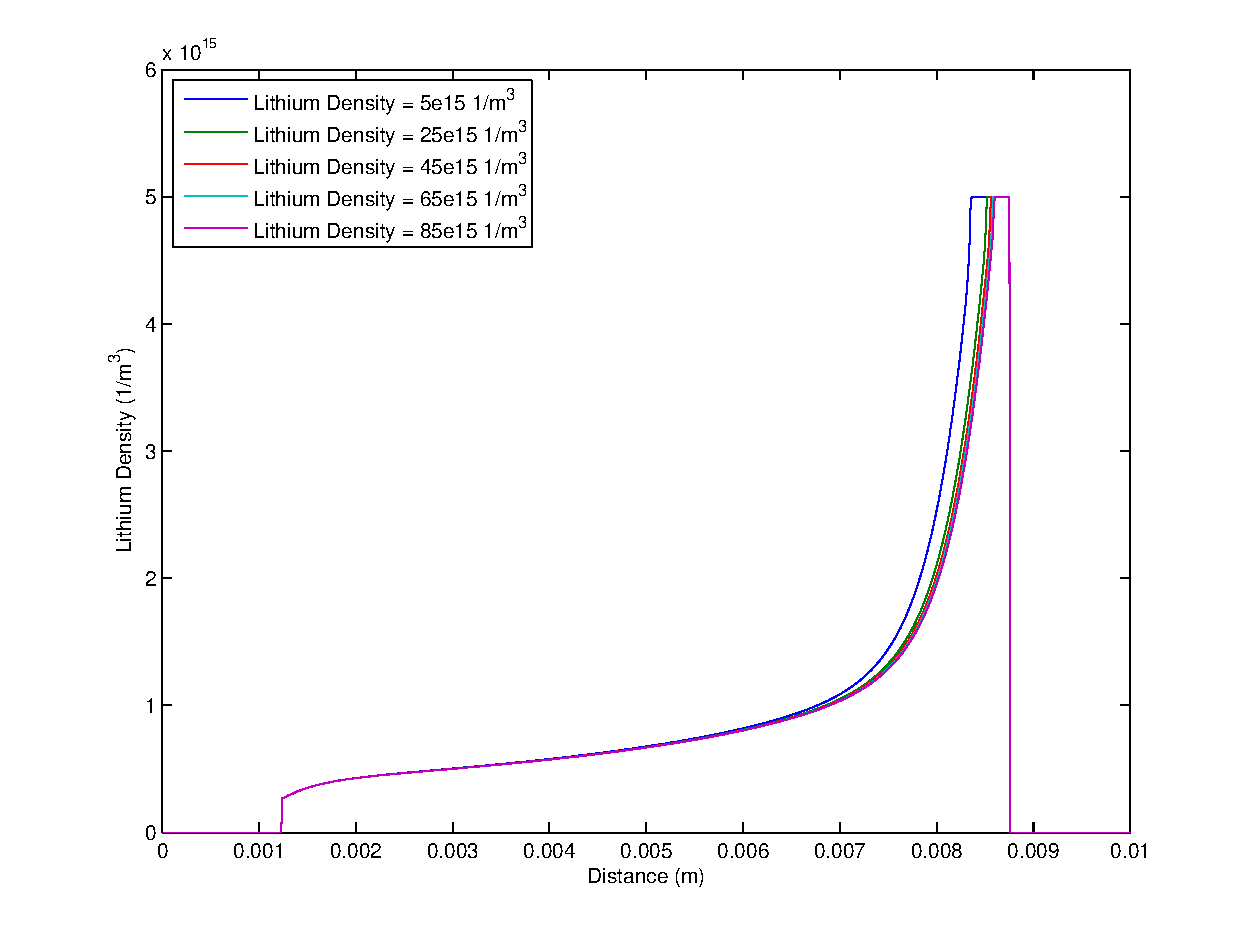
\includegraphics[scale=0.50]{LithiumDiff}
\caption{Normalized lithium densities at steady state} 
\label{LithiumDiff}
\end{figure}

First few miliseconds of this simulation was run without the movement of lithium ions. At this stage normalized currents are identical to each other which means a simulation with low density can be scaled up to any density without introducing any error. The introduction of lithium ions slowly deviates the current plots from each other over time but the overall behavior of the memristor remains unchanged. The current density decreases over time and reaches a steady state value. After the first plot which has the lowest hole density, consecutive plots get closer and they are almost impossible to distinguish from each other at steady state.

\begin{figure}[!htp]
\centering
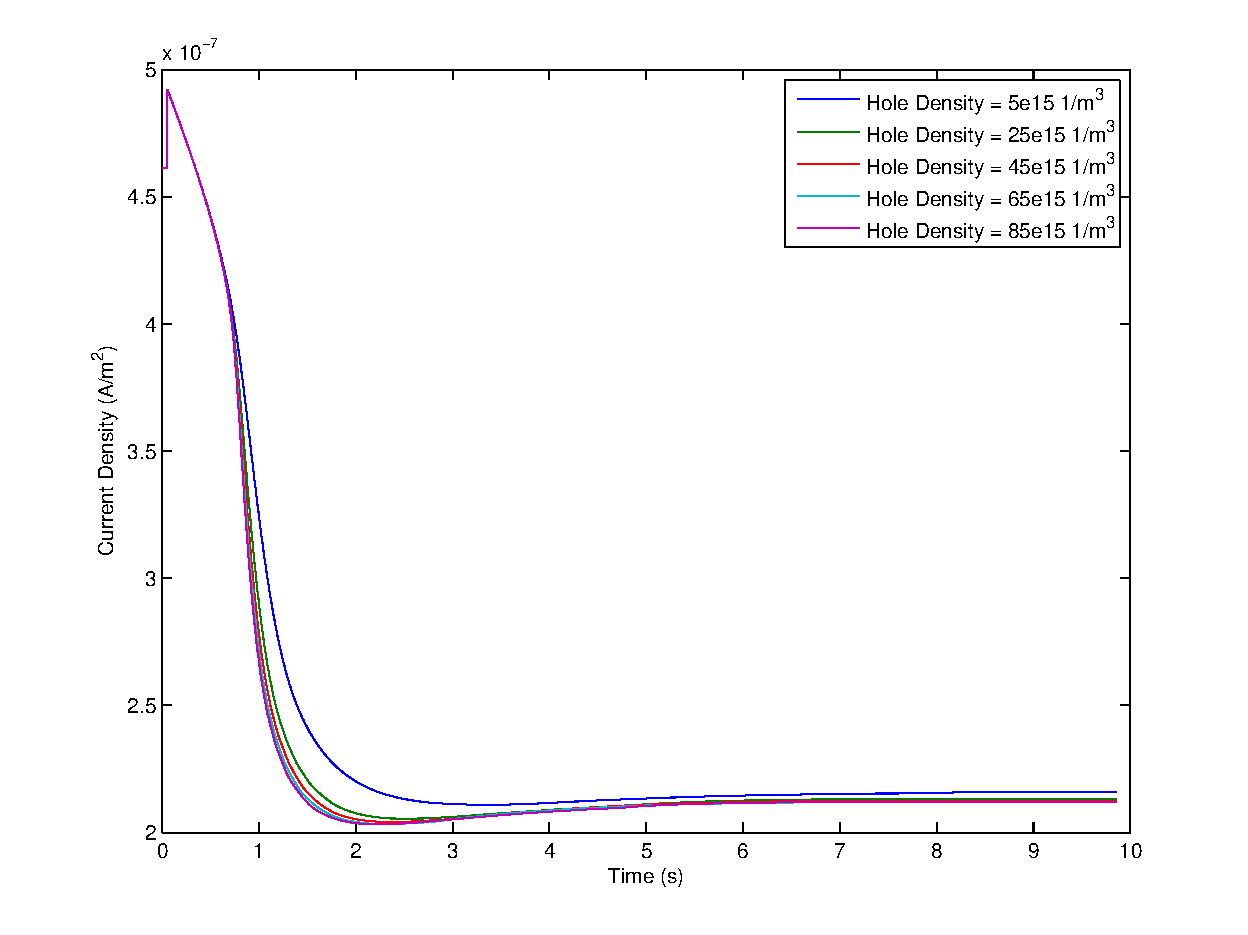
\includegraphics[scale=0.50]{DensityDiff}
\caption{Normalized hole current densities} 
\label{DensityDiff}
\end{figure}

The impact of increasing charge density can be numerically explored using normalized plots. Following formula was used to calculate a percentage difference between different normalized carrier densities as well as normalized current densities. 


\begin{equation}
\centering
P_i = \frac{1}{ K}\sum_{k=1}^{K}\lvert 100 \;\frac{n_{i}(x_k)/r-n_{0}(x_k)}{n_{0}(x_k)}\rvert
\end{equation}

\begin{equation}
\centering
P_i = \frac{1}{ T}\sum_{k=1}^{T}\lvert 100 \;\frac{J_{i}(t_k)/r-J_{0}(t_k)}{J_{0}(t)}\rvert
\end{equation}


K is for total number of points along x axis and T is the total number of time steps taken by the simulator. $x_{k}$ and $t_{k}$ are used to for a point in x axis and a point in time respectively. r is the normalization constant described in equation \ref{NormConst}. Both equations start by taking a point in either space (lithium/hole density) or time (current density) for a simulation with a certain carrier density and normalize them. After that point is normalized its difference from the lowest carrier density simulation is calculated as a percentage. Finally all the differences are averaged and used as a measure of the difference between simulations with different charge densities. They can also be used as an approximate error during scaling. 

\begin{figure}[!htp]
\centering
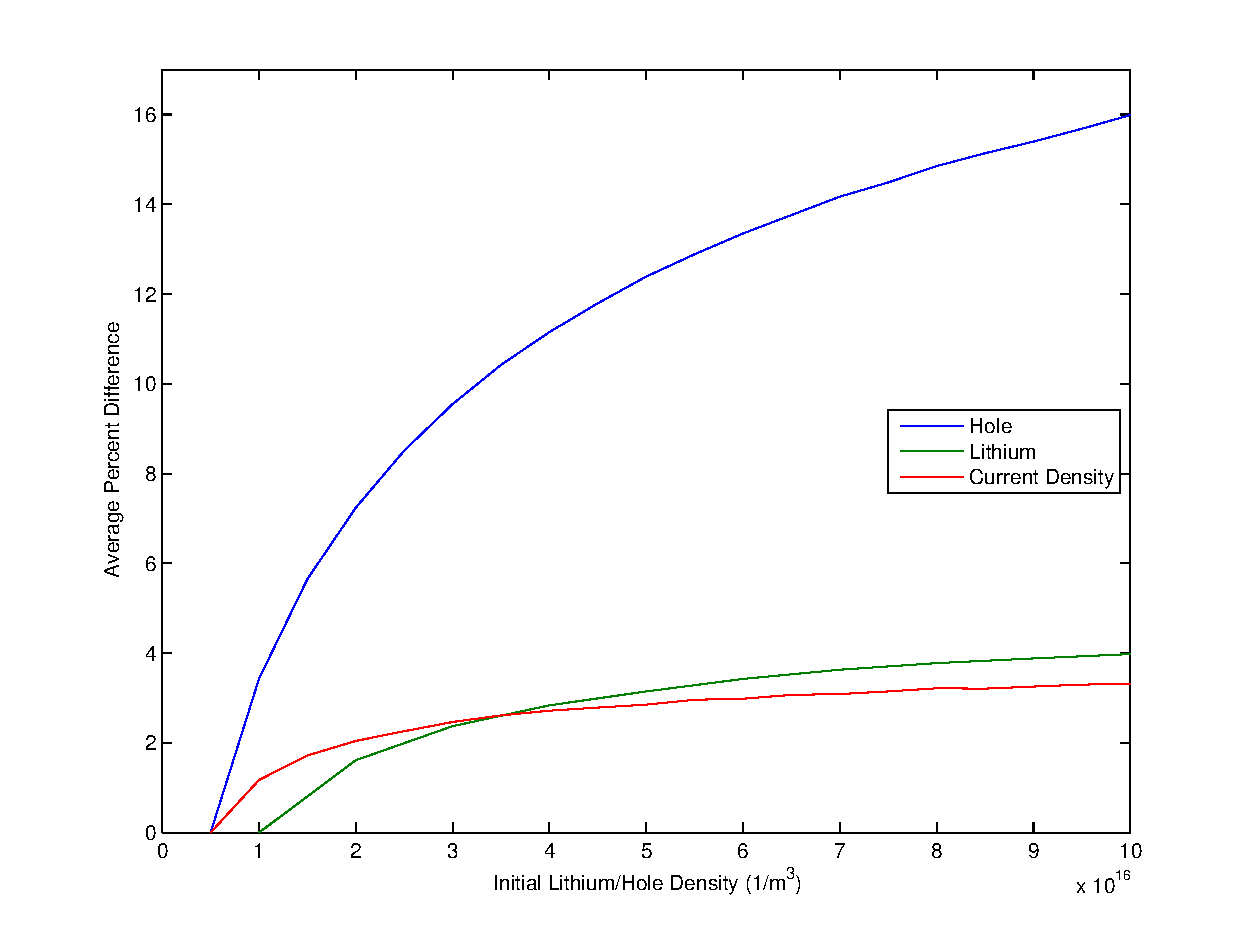
\includegraphics[scale=0.50]{AllDiff}
\caption{Average difference for hole lithium and current densities for various initial hole densities} 
\label{AllDiff}
\end{figure}

Figure \ref{AllDiff} shows the difference hole/lithium density makes in the simulation. Carrier densities in the dry regions of the PEODT change very little between consecutive simulations since lithium ions do not reach there. For this reason only the densities at the wet PEDOT were used to measure the difference between plots. 

In all 3 cases, there is an increase in average difference for increasing carrier density. Hole density shows the most difference between plots. Since holes are free to move inside the PEDOT they directly get effected by the change in debye length due to the increase in hole density. This is not the case for lithium ions because their movement is restricted by the limit on lithium density. In contrast, current density is not as sensitive to density changes as lithium and hole distributions.

 An approximate error estimation can be made for current density if a low hole/lithium density is used for simulation and then scaled up to match the actual memristor. Figure \ref{AllDiff} shows around 3.3 \% difference for 2 orders of magnitude increase in hole density. Assuming the error scales linearly after that point a total of 6 orders of magnitude will result in 9.9 \% error introduced in order to linearly scale from $10^{15}$ to $10^{21}$. The actual error is likely to be less since the error progresses sub linearly. Following the same procedure 6 orders of magnitude difference produces a 12 \% error for lithium distribution and 48 \% error for hole distribution. The difference in hole distribution looks very large but the overall shape of the plot is still reserved, most change occurs around the wet/dry PEDOT interface where lithium accumulates. Based on these error margins and previous plots it can be concluded that the behavior of the memristor simulated using low charge density is very similar to the simulation at high carrier density.    




\end{doublespace}
